
 
\documentclass[pdflatex,sn-nature]{sn-jnl}% Style for submissions to Nature Portfolio journals
%%documentclass[pdflatex,sn-basic]{sn-jnl}% Basic Springer Nature Reference Style/Chemistry Reference Style
%%\documentclass[pdflatex,sn-mathphys-num]{sn-jnl}% Math and Physical Sciences Numbered Reference Style 
%%\documentclass[pdflatex,sn-mathphys-ay]{sn-jnl}% Math and Physical Sciences Author Year Reference Style
%%\documentclass[pdflatex,sn-aps]{sn-jnl}% American Physical Society (APS) Reference Style
%%\documentclass[pdflatex,sn-vancouver,Numbered]{sn-jnl}% Vancouver Reference Style
%%\documentclass[pdflatex,sn-apa]{sn-jnl}% APA Reference Style 
%%\documentclass[pdflatex,sn-chicago]{sn-jnl}% Chicago-based Humanities Reference Style

%%%% Standard Packages
%%<additional latex packages if required can be included here>


\usepackage{amsmath,amssymb,amsfonts}%
\usepackage{amsthm}%
\usepackage{mathrsfs}%
\usepackage[title]{appendix}%
\usepackage{xcolor}%
\usepackage{textcomp}%
\usepackage{manyfoot}%
\usepackage{booktabs}%


%
\usepackage{amsmath,amsfonts}
\usepackage{algorithmic}
\usepackage{array}
\usepackage[caption=false,font=normalsize,labelfont=sf,textfont=sf]{subfig}
\usepackage{textcomp}
\usepackage{stfloats}
\usepackage{url}
\usepackage{verbatim}
\usepackage{graphicx}
\usepackage{enumerate}
\usepackage{listings}
\usepackage{hyperref}
\usepackage{xspace}
\usepackage{balance}
\usepackage[most]{tcolorbox}
\usepackage{awesomebox}
\usepackage{multirow}
\usepackage{blindtext}



%%%%

%%%%%=============================================================================%%%%
%%%%  Remarks: This template is provided to aid authors with the preparation
%%%%  of original research articles intended for submission to journals published 
%%%%  by Springer Nature. The guidance has been prepared in partnership with 
%%%%  production teams to conform to Springer Nature technical requirements. 
%%%%  Editorial and presentation requirements differ among journal portfolios and 
%%%%  research disciplines. You may find sections in this template are irrelevant 
%%%%  to your work and are empowered to omit any such section if allowed by the 
%%%%  journal you intend to submit to. The submission guidelines and policies 
%%%%  of the journal take precedence. A detailed User Manual is available in the 
%%%%  template package for technical guidance.
%%%%%=============================================================================%%%%

%% as per the requirement new theorem styles can be included as shown below
\theoremstyle{thmstyleone}%
\newtheorem{theorem}{Theorem}%  meant for continuous numbers
%%\newtheorem{theorem}{Theorem}[section]% meant for sectionwise numbers
%% optional argument [theorem] produces theorem numbering sequence instead of independent numbers for Proposition
\newtheorem{proposition}[theorem]{Proposition}% 
%%\newtheorem{proposition}{Proposition}% to get separate numbers for theorem and proposition etc.

\theoremstyle{thmstyletwo}%
\newtheorem{example}{Example}%
\newtheorem{remark}{Remark}%

\theoremstyle{thmstylethree}%
\newtheorem{definition}{Definition}%

\raggedbottom
%%\unnumbered% uncomment this for unnumbered level heads

\newtcbtheorem{obs}{Finding}{%
        theorem name,%
        colback=gray!5,%
        colframe=gray!35!black,%
        fonttitle=\bfseries,title after break={Lemma  -- \raggedleft Continued}%
    }{lem}

\newcommand{\tb}[2]{\tipbox{{\bf Finding #1}. #2}}

\newcommand{\droidxp}{DroidXP\xspace}
\newcommand{\review}[1]{\textcolor{black}{#1}}
\newcommand{\alert}[1]{\textcolor{red}{#1}}
\newcommand\kn[1]{\textcolor{red}{KN: #1}}
\newcommand\fh[1]{\textcolor{blue}{FH: #1}}
\newcommand\rb[1]{(\textcolor{red}{RB: #1})}

\newcommand{\highlight}[1]{{\color{red}}#1}

\newcommand\raw[1]{\textcolor{red}{#1}\xspace}

\newcommand{\mas}{MAS approach\xspace}

\newcommand{\fm}[1]{\emph{#1}\xspace}

\newcommand{\gps}{\fm{gappusin}}  % the gappusin family.

\newcommand{\rmb}{\fm{revmob}} 

\newcommand{\sscore}{Similarity Score\xspace}

\newcommand{\rqa}{What is the impact of considering a larger and diverse dataset on the accuracy of the \mas for malware classification?}

\newcommand{\rqb}{How much gain we obtain on the performance of the \mas for malware classification when considering trace analysis?}

\newcommand{\rqc}{What is the influence of the similarity between the original and repackaged
                  versions of the apps on the performance of the \mas for malware classification?}

\newcommand{\rqd}{What is the influence of the malware family (e.g., \fm{gappusin}, \fm{kuguo}, \fm{dowgin}) on the performance of the \mas for malware classification?}

\newcommand{\rqe}{How much gain we obtain on the performance of the \mas for malware classification when considering its extensions?}


\newcommand{\repack}{RePack\xspace}
\newcommand{\amc}{AndroMalPack\xspace}

\newcommand{\appsSmall}{102\xspace}
\newcommand{\apps}{\textcolor{black}{4,076}\xspace}
\newcommand{\napps}{\textcolor{blue}{726}\xspace}

\newcommand{\sds}{\texttt{SmallDS}\xspace}
\newcommand{\cds}{\texttt{LargeDS}\xspace}
\newcommand{\nds}{\texttt{DS3}\xspace}
\newcommand{\avt}{\texttt{avclass2} tool\xspace}
\newcommand{\vt}{\texttt{VirusTotal}\xspace}
\newcommand{\se}{security engine\xspace}
\newcommand{\ses}{security engines\xspace}


\newcommand{\fone}{F1-score\xspace}
\newcommand{\fscoreSmall}{0.89\xspace}
\newcommand{\fscoreNew}{0.85\xspace}

\newcommand{\nfscoreSmall}{0.85\xspace}
\newcommand{\nfscoreSmallC}{0.87\xspace}

\newcommand{\fscore}{\textcolor{black}{0.54}\xspace}
\newcommand{\fscoreC}{\textcolor{blue}{0.49}\xspace}

\newcommand{\malwares}{\textcolor{black}{2,895}\xspace}
\newcommand{\malwaresP}{\textcolor{black}{71.02}}
\newcommand{\malwaresN}{\textcolor{blue}{87.98}}
\newcommand{\appsGps}{\textcolor{black}{1,337}\xspace}
\newcommand{\appsGpsFN}{\textcolor{black}{1,170}\xspace}



\begin{document}

\title[The Achilles' Heel of the Android Mining Sandbox Approach for Malware Identification
]{The Achilles' Heel of the Android Mining Sandbox Approach for Malware Identification
}

%%=============================================================%%
%% GivenName	-> \fnm{Joergen W.}
%% Particle	-> \spfx{van der} -> surname prefix
%% FamilyName	-> \sur{Ploeg}
%% Suffix	-> \sfx{IV}
%% \author*[1,2]{\fnm{Joergen W.} \spfx{van der} \sur{Ploeg} 
%%  \sfx{IV}}\email{iauthor@gmail.com}
%%=============================================================%%

\author*[1]{\fnm{Francisco} \sur{Costa}}\email{francisco.costa@aluno.unb.br}

\author[1]{\fnm{Ismael} \sur{Medeiros}}\email{ismael.medeiros@aluno.unb.br}
\equalcont{These authors contributed equally to this work.}

\author[1]{\fnm{Leandro} \sur{Oliveira}}\email{leandro.oliveira@aluno.unb.br}
\equalcont{These authors contributed equally to this work.}

\author[1]{\fnm{Jo\~{a}o} \sur{Cal\'{a}ssio}}\email{joao.calassion@aluno.unb.br}
\equalcont{These authors contributed equally to this work.}

\author[1]{\fnm{Rodrigo} \sur{Bonif\'{a}cio}}\email{rbonifacio@unb.br}
\equalcont{These authors contributed equally to this work.}

\author[2]{\fnm{Krishna} \sur{Narasimhan}}\email{kri.nara@informatik.tu-darmstadt.de}
\equalcont{These authors contributed equally to this work.}

\author[2]{\fnm{Mira} \sur{Mezini}}\email{mezini@informatik.tu-darmstadt.de}
\equalcont{These authors contributed equally to this work.}

\author[3]{\fnm{M\'{a}rcio} \sur{Ribeiro}}\email{marcio@ic.ufal.br}
\equalcont{These authors contributed equally to this work.}

\affil*[1]{\orgdiv{Computer Science Department}, \orgname{University of Bras\'{i}lia}, \orgaddress{\city{Bras\'{i}lia}, \country{Brazil}}}

\affil[2]{\orgdiv{Software Technology Group}, \orgname{TU Darmstadt}, \orgaddress{\city{Darmstadt}, \country{Germany}}}

\affil[3]{\orgdiv{Computing Institute}, \orgname{ Federal University of Alagoas}, \orgaddress{\city{Macei\'{o}},  \country{Brazil}}}

%%==================================%%
%% Sample for unstructured abstract %%
%%==================================%%

\abstract{The widespread use of smartphones in our daily lives has elevated concerns regarding their security among researchers and practitioners.
Particularly, security issues are highly prevalent in Android, the most popular mobile operating system. Previous research has explored
various techniques to address these concerns, including the Mining Android Sandbox approach (\mas), which aims to identify malicious behavior in repackaged Android applications (apps).
However, earlier studies have been limited by small datasets, typically consisting of only \appsSmall pairs of original and repackaged apps.
This limitation raises questions about the external validity of their findings and whether the MAS approach can be generalized to larger datasets.
To address these concerns, this paper presents the results of an experiment that replicates state-of-the-art research on evaluating the
accuracy of the \mas. Unlike previous studies, our research employs a dataset that is an order of magnitude larger, comprising \apps
pairs of apps covering a more diverse range of Android malware families. Surprisingly, our findings indicate a significant drop in the accuracy of the MAS approach for identifying malware, with
the \fone decreasing from \fscoreSmall in previous studies to \fscore in our larger dataset. Upon closer examination, \review{we discovered that the higher representation of certain malware families partially accounts for the increased number of instance} where the \mas fails to correctly classify a repackaged app as malware. Our findings highlight the limitations of the MAS approach, particularly when scaled, and underscore the importance of complementing it with other techniques to effectively detect a
broader range of malware. This opens avenues for further discussion on addressing the blind spots
that affect the accuracy of the \mas.}



\keywords{Android Malware Detection, Dynamic Analysis, Mining Android Sandboxes.}

%%\pacs[JEL Classification]{D8, H51}

%%\pacs[MSC Classification]{35A01, 65L10, 65L12, 65L20, 65L70}

\maketitle

\section{Introduction}\label{sec:introduction}

Mobile technologies like smartphones and tablets have become fundamental to the way we function as a society. Almost two-thirds of the world population
uses mobile technologies~\cite{Comscore,DBLP:journals/tse/MartinSJZH17}, with the
Android Platform dominating this market and accounting for more than 70\% of the \emph{mobile
market share}, with almost 2.5 million Android applications~\footnote{In this paper, we will use the terms Android Applications, Android Apps, and Apps interchangeably, to refer to Android software applications} (apps)
available on the Google Play Store, in June 2023~\cite{Statista}.  
As popularity rises, so does the risk of potential attacks, prompting collaborative efforts from both academia and industry to design and develop new techniques for identifying malicious behavior or vulnerable code in Android apps~\cite{10.1145/3017427}.

For instance, one popular class of Android malware is based on repackaging apps~\cite{DBLP:conf/wcre/BaoLL18,DBLP:conf/iceccs/LeB0GL18} where a benign
version of an app is
%such as Google Play, 
infected with malicious code, e.g., to broadcast
sensitive information to a private server~\cite{DBLP:journals/tse/LiBK21}, and subsequently shared
with users using even official app stores. The Mining Android Sandbox approach (\mas) was initially designed to construct sandboxes based on exploratory calls to sensitive APIs~\cite{DBLP:conf/icse/JamrozikSZ16}. However, it has also proven effective in detecting Android repackaged malware. The \mas operates in two distinct phases. In the first phase (exploratory phase), it utilizes automated test case generation tools to abstract the behavior of an app, focusing on calls to sensitive APIs (Application Programming Interfaces). Subsequently, during the normal executions of the app, the generated sandbox blocks any calls to sensitive APIs not observed during the exploratory phase.

Prior studies~\cite{DBLP:conf/wcre/BaoLL18,DBLP:journals/jss/CostaMMSSBNR22} have investigated the application of the MAS approach in detecting potential malicious behavior in repackaged apps. These studies have also conducted comparisons of the approach's performance by employing different test case generation tools during the exploratory phase, including Monkey~\cite{Monkey}, DroidBot~\cite{DBLP:conf/icse/LiYGC17}, and Droidmate~\cite{DBLP:conf/kbse/BorgesHZ18}.
These studies provide evidence that DroidBot surpasses other test generation tools, uncovering a larger number of potential malicious behaviors.
But these previous studies have two main limitations.
First, they use a small dataset of malware comprising only \appsSmall pairs of original/repackaged versions of an app---compromising external validity. Second, their assessments do not investigate
the impact of relevant features of the repackaged apps on the accuracy of the \mas for malware classification, including
(a) whether or not the repackaged version is a malware, (b) the similarity between the original and the repackaged versions of an app,
and (c) the malware family (e.g., \fm{gappusin}, \fm{kuguo}, \fm{dowgin}, etc.) when the repackaged
version of an app is a malware. This limitations compromise a full understanding of the \mas performance. We present more details about the \mas and related work in Section~\ref{sec:background}.


To understand the impact of these issues on results already published in the literature, in this paper we reconsider the accuracy of the \mas based on
DroidBot~\cite{DBLP:conf/icse/LiYGC17}---as we mentioned, the test case generation tool that, according to the literature, leads to the most accurate Android sandbox, regarding malware identification. 
Compared to previous studies~\cite{DBLP:conf/wcre/BaoLL18,DBLP:conf/scam/CostaMCMVBC20},
we use a curated dataset of app pairs (original/repackaged versions) that is, in terms of magnitude, larger than the previously used
dataset (it contains \apps pairs of original/repackaged apps). We detail our datasets and the procedures we follow for data collection and data analysis in Section~\ref{sec:experimentalSetup}.
 
{\bf Negative results.} Our study reveals a significantly lower
accuracy (\fone of \fscore) of the \mas in comparison to what has been reported before (\fone of \fscoreSmall). 
Since an accuracy of \fscore is clearly unsatisfactory for a trustworthy malware classification technique, we conduct a set of experiments 
to understand the reasons for the lower accuracy in our larger dataset.
Our further assessments reveal that the \mas fails to correctly classify most samples from a specific set of malware families, particularly those from the \gps family (a particular class of adware that frequently appears in repackaged apps). Out of the total of \appsGps samples within this family in our large dataset, the \mas failed to correctly classify \appsGpsFN samples as malware. Accordingly, these families are responsible for substantially reducing the recall of the \mas. We detail the results of our experiments in Section~\ref{sec:results}. 

We also discuss the implications and possible threats to the validity of our study in Section~\ref{sec:discussion} and present some final remarks in Section~\ref{sec:conclusions}. 
The main artifacts we produced during this research are available in the paper repository.

\begin{small}
  \begin{center}
    \url{https://github.com/droidxp/paper-droidxptrace-results}
  \end{center}
\end{small}


\section{Background and Related Work}\label{sec:background}

%% In this section, we introduce the concepts and terminology that are necessary to understand the reminder of this paper. First, Section~\ref{sec:sand} introduces some background information about \emph{sandboxes} within the security context. Section~\ref{sec:repackage} presents background information about repackaged application and how they introduce malicious behavior.
%% Finally, in Section~\ref{sec:android-sandbox} we review the \emph{mining sandbox approach} for detecting repackaged Android apps.

There are many tools that favor developers to reverse engineering the Android bytecode language~\cite{DBLP:conf/issta/WangGMC15}.
For this reason, software developers can easily decompile trustworthy apps, modify their contents by inserting malicious code,
repackage them with malicious payloads, and re-publish them in app stores, including official ones like the Google Play Store.
It is well-known that repackaged Android apps can leverage the popularity of real apps to increase their propagation and spread malware~\cite{DBLP:journals/tse/LiBK21}. As an example, in 2016 a repackaged version of the famous Pokémon Go app was discovered less than 72 hours after the game was officially released in the United States, Australia, and New Zealand~\cite{DBLP:journals/tse/LiBK21}. The repackaged version, originated from an unofficial app store, gained full control over the victim's phone, obtaining access to main functions such as the phonebook, audio recorder, and camera.

Repackaging has been raised as a noteworthy security concern in Android ecosystem by stakeholders in the app development industry and researchers~\cite{DBLP:journals/ese/KhanmohammadiEH19}. Indeed, there are reports claiming that about 25\% of Google Play Store app content correspond to repackaged apps~\cite{DBLP:conf/sigmetrics/ViennotGN14}. Nevertheless, all the workload to detect and remove malware from markets by the stores (official and non-official ones), have not been accurate enough to address the problem. As a result, repackaged Android apps threaten security and privacy of unsuspicious Android app users, beyond compromising the copyright of the original developers~\cite{DBLP:journals/access/KimLCP19}. Aiming at
mitigating the threat of malicious code injection in repackaged apps,
several techniques based on both static and dynamic analysis of Android apps have been proposed,
including the \mas for malware classification~\cite{DBLP:conf/icse/JamrozikSZ16,DBLP:conf/wcre/BaoLL18}. 





\subsection{Mining Android Sandboxes}\label{sec:android-sandbox}

A \emph{sandbox}
is a well-known mechanism to secure a system and forbid a software component from accessing
resources without appropriate permissions. Sandboxes have also been used to build an isolated
environment within which applications cannot affect other programs, the network, or other device
data~\cite{DBLP:journals/peerj-cs/MaassSCS16}. The idea of using sandboxes emerged from the
need to test unsafe software, possible malware, without worrying about the integrity of the
device under test~\cite{DBLP:conf/esorics/BordoniCS17}, shielding the operating system from security issues.
To this end, a sandbox environment should have the minimum requirements to run the
program, and make sure it will never assign the program more privileges than it should have,
respecting the \emph{least privilege} principle.
% This principle ensures unauthorized access to resources,
% improving the system's overall health.
Within the Android ecosystem, sandbox approaches ensure the principle
of the \emph{least privilege} by preventing apps from having direct access to resources like device hardware (e.g., GPS, Camera), or sensitive data from other apps. Access to sensitives data
like contact list or resources are granted through specific APIs, known as sensitive APIs, which are managed by by coarse-grained Android permissions system~\cite{DBLP:journals/corr/abs-2109-06613}.



%% The main market source for Android apps is Google Play Store. Unfortunately, it has
%% a flexible policy regarding the process of publishing apps, and therefore, many Android apps are removed from the
%% store because of issues related to malware\cite{DBLP:conf/msr/WangLL0X18}. Google Play tries
%% to minimize unauthorized access to sensitive resources by malicious apps,
%% listing each app with its requested permission. {\color{red}Those permissions are presented to Android
%% users at app installation moment since version 6}. However, some works presented that most users are careless regarding these permissions since they are only interested to run the app~\cite{DBLP:conf/soups/FeltHEHCW12}. This represents a great security breach since malware usually asks for more permissions than their APIs normally would require~\cite{DBLP:conf/ccs/FeltCHSW11}.

%% \begin{figure}[ht]
%% \centering
%% 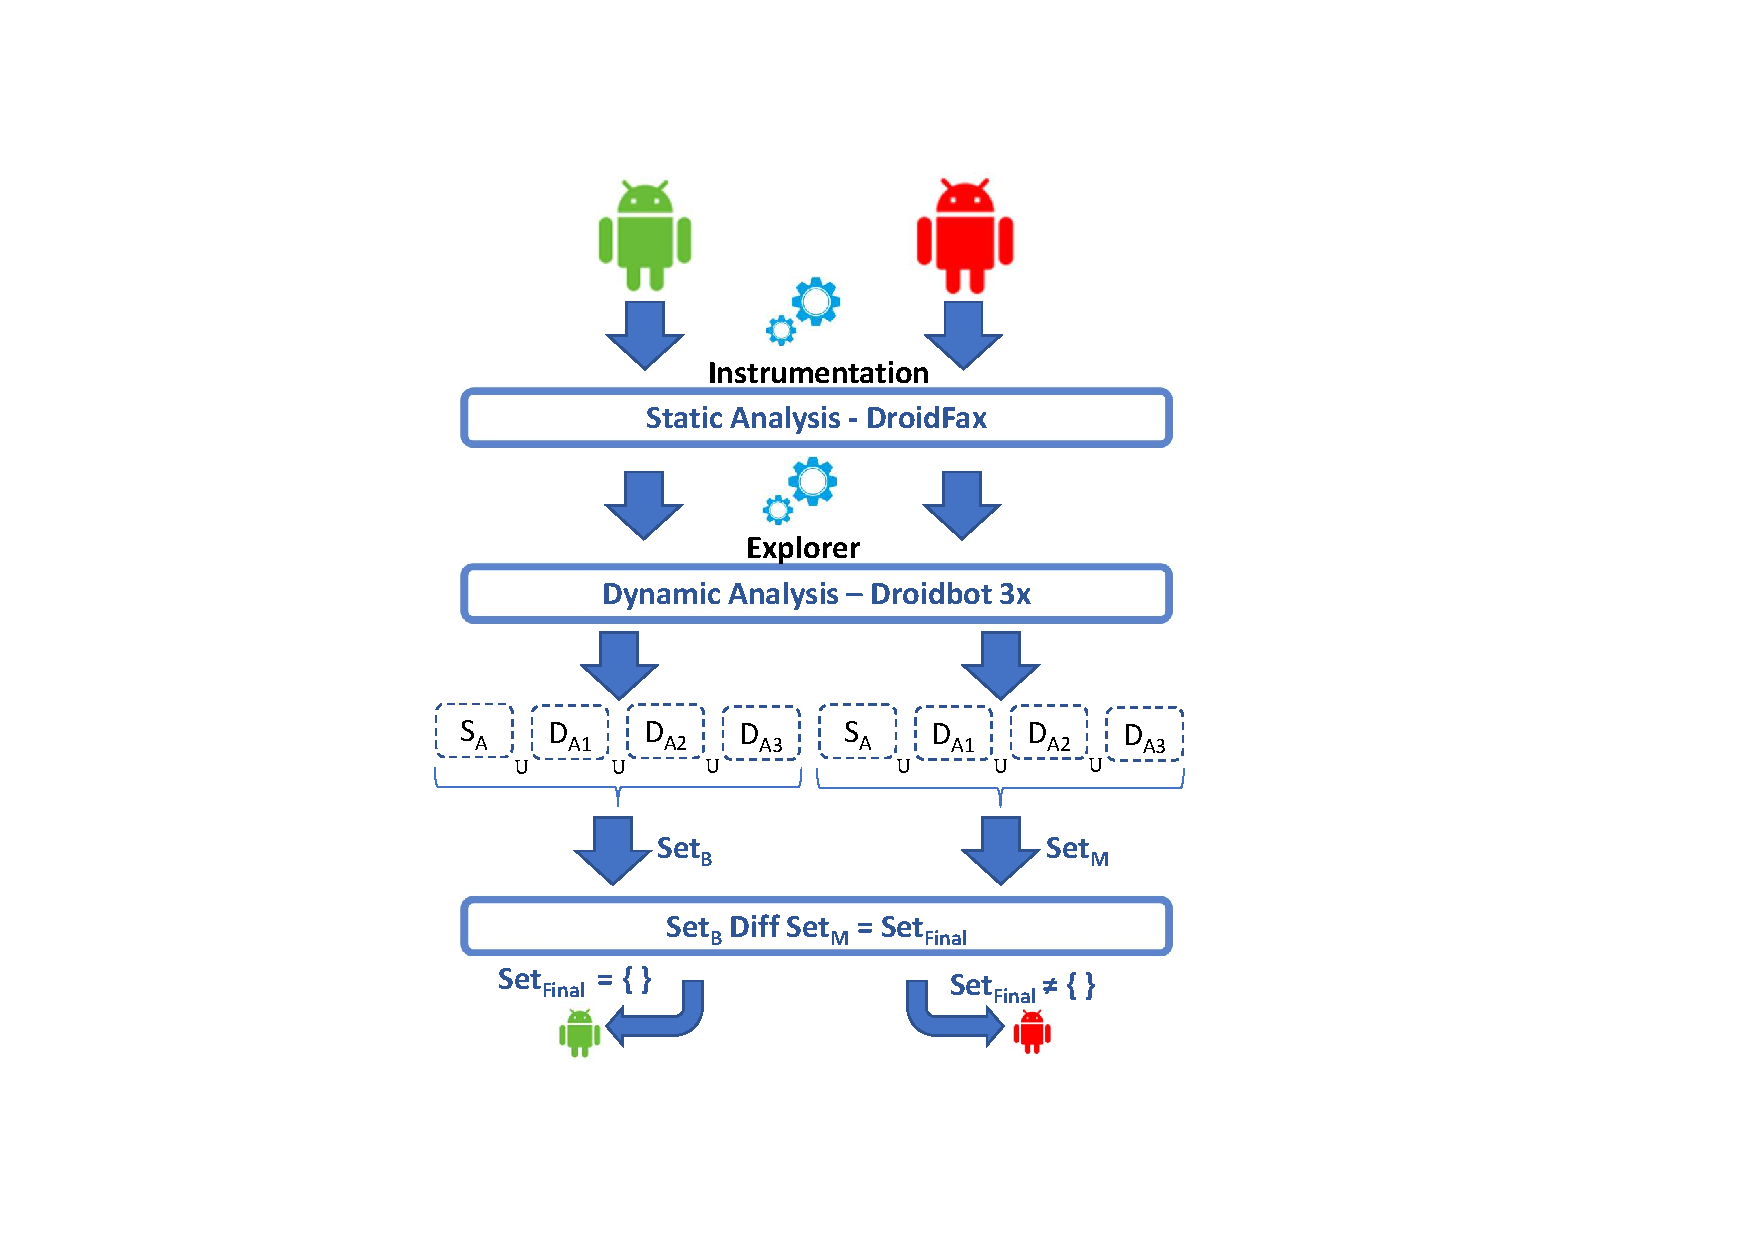
\includegraphics[scale=0.35]{images/mineSandbox.pdf}
%% \caption{Mine Sandbox.}
%%  \label{fig:mineSandbox}
%% \end{figure}

The \mas~\cite{DBLP:conf/icse/JamrozikSZ16} aims at automatically
building a sandbox through dynamic analysis (i.e., using automatic test generation tools).
The main idea is to grant permissions to an app based on its calls to sensitive APIs.
Thus, sandboxes build upon these calls to create safety rules and then block future
calls to other sensitive resources, which diverge from those found in the first exploratory
phase. Using the Droidmate test generation tool~\cite{DBLP:conf/icse/JamrozikZ16},
Jamrozik et al. proposed a full-fledged
implementation of the \mas, named Boxmate~\cite{DBLP:conf/icse/JamrozikSZ16}. 
Boxmate records the occurrences of calls to sensitive APIs and, optionally, the UI
events (e.g., a button click) that trigger these calls. Therefore, it is possible to configure Boxmate to record events associated with each sensitive call as
tuples (event, API), instead of recording just the set of calls to sensitive APIs. Jamrozik et al. argue that, in this way, Boxmate generates finer
grain results, which
might improve the accuracy of the \mas---even with the presence of reflection, a feature commonly used in
malicious apps~\cite{DBLP:conf/issta/0029BOK16}.

In fact, the \mas can be implemented using
a mix of static and dynamic analysis. In the first phase, one
can instrument an Android app to log any call to the Android sensitive methods.
After that, one can execute a test case generation tool (such as DroidMate, DroidBot, or Monkey) to explore the app behavior at runtime,
while the calls to sensitive APIs are recorded.
%Figure~\ref{fig:mineSandbox} presents this general approach for \mas.
This set of calls to sensitive APIs is then used
to configure the sandbox. The general \mas % (see Figure~\ref{fig:mineSandbox})
suggests that the more efficient the test generation tool (for instance, in terms of code coverage),
the more accurate would be the resulting sandbox.


%\todo[inline]{Since this figure is not discussed in the paper, we can remove it without any problem. I have enriched the previous paragraph, though, to make it
%  more necessary. Nonetheless, I will change this figure a bit, in order to
%represent the instrumentation phase.}

\subsection{Mining Android Sandbox for Malware Classification}

Besides being used to generate Android sandboxes, the \mas is also effective 
to detect if a repackaged version of an Android app contains malicious
behavior~\cite{DBLP:conf/wcre/BaoLL18}. In this scenario, the \emph{effectiveness} of the approach
is estimated in terms of the accuracy in which malicious behavior is correctly identified in the repackaged version of the
apps.


%Figure~\ref{fig:sensitiveAPI} illustrates the \mas for
%repackaged apps identification.
%We leverage DroidXP~\cite{DBLP:conf/scam/CostaMCMVBC20} to collect the set of sensitive APIs
%the versions of the apps call (benign/malign versions).
The \mas for malware classification typically works as follows. In a first step ({\bf instrumentation phase}), 
a tool instruments the code of the apps (both original and repackaged versions) to collect relevant information
during the apps execution in later stages. Then, in a second step ({\bf exploration phase}),
the \mas collects a set $S_1$ with all calls to sensitive APIs the original version of an app executes while running a test case generator tool (like DroidBot).
In the third step ({\bf exploitation phase}), the \mas (a) collects a set $S_2$ with all calls to sensitive APIs the repackaged version of an app
executes while running a test case generator tool and then (b) computes the set $S = S_2 \setminus S_1$ and checks whether  $S$ is empty or not.
The \mas classifies the repackaged version as a malware whenever $|S| > 0$.  

%%We configure DroidXP to run DroidBot for $3$ minutes. Since some malware may use dynamic features (such as reflection) to introduce malicious behavior,
%%which can change apps behavior at runtime~\cite{DBLP:journals/spe/ZhangLTX18,DBLP:journals/tosem/LiTX19}, this second
%%analysis is also important to disclose some sensitive APIs calls ignored by first analysis (static analysis).

%%While our static analysis is made once, we execute dynamic analysis $3$ times. The result of static analysis and all executions is finally joined, forming a final set containing all calls to sensitive APIs coming from the original version of the app, as described at Figure~\ref{fig:sensitiveAPI}: ($S_{A}$, $D_{A1}$, $D_{A2}$, $D_{A3}$). We carry out the same procedure for the malicious version of the apps, creating a distinct set of calls to sensitive APIs (now coming from the malicious version of the apps). In a final step, we compare the two sets of calls to sensitive APIs ($Set_B, Set_M$). We use the following rules to check for a malicious behavior. 

%% \begin{enumerate}
%%     \item If the difference between the two final sets is an empty set, we cannot distinguish the benign from the malicious version of the app (false negative).
%%     \item Otherwise, we successfully distinguish the benign from the malicious version of the app (true positive). 
%%     %\kn{Cant we replace the first part of the second point simply as "Otherwise" or is there some specific corner cases that I am missing}
%% \end{enumerate}

%% In addition, this procedure also enables us to identify the calls to sensitive APIs that are more frequently injected by the malicious version of the apps
%% in our dataset. 

%% %\fh{here I have to insert the figure}

%%\begin{figure}[ht]
%%\centering
%%\includegraphics[scale=0.45]{images/sensitiveAPIdiff.pdf}
%%\caption{All procedure for suspicious app identification %%using sensitive API set diff.}
%%\label{fig:sensitiveAPI}
%%\end{figure}



%\kn{I have commented out the subsection here as it seems redundant with the previous subsection}
%\subsection{The Mining Android Sandbox Approach for Malware Identification}

%The focus of our paper is in approaches that mine android sandboxes to classify Android Malware.
%There is a vast body of research in this direction. 

Previous research works reported the results of empirical studies that aim to investigate the effectiveness of
the \mas for malware classification~\cite{DBLP:conf/wcre/BaoLL18,DBLP:conf/scam/CostaMCMVBC20}.
For instance, Bao et al. found that, in general, the sandboxes constructed using test generation tools classify at least 66\% of repackaged apps as malware in a
dataset comprising 102 pairs of apps (original/repackaged versions)~\cite{DBLP:conf/wcre/BaoLL18}.
Actually, the mentioned work performed two studies: one pilot study involving a dataset
of 10 pairs of apps (\texttt{SmallE}), in which the authors executed each test case generation tools for one hour; and a larger experiment
(\texttt{LargeE}) involving 102 pairs of
apps in which the authors executed the test case generation tools for one minute~\cite{DBLP:conf/wcre/BaoLL18}.

Here we replicate their larger experiment. 
The authors also presented that, among five test generation tools used, DroidBot~\cite{DBLP:conf/icse/LiYGC17} leads to the most effective sandbox.
Le et al. extend the \mas for malware classification with additional verification,
such as the values of the actual parameters used in the
calls to sensitive APIs~\cite{DBLP:conf/iceccs/LeB0GL18}, while
Costa et al.\cite{DBLP:journals/jss/CostaMMSSBNR22} investigated the impact of static analysis to complement the accuracy of the \mas
for malware classification. Their study reports that DroidFax~\cite{DBLP:conf/icsm/CaiR17a}, the static analysis infrastructure used in~\cite{DBLP:conf/wcre/BaoLL18}, classifies as malware almost half of the repackaged apps.

%\rb{For a TSE paper, we should include an additional section
%summarizing the research on Android malware classification.}

\subsection{Android Malware Classification - State-of-the-art}

The field of malware detection for the Android platform is fertile, with a significant number of secondary studies already published~\cite{DBLP:conf/eann/SerajPP22,DBLP:conf/icsoft/LekssaysFA20,DBLP:journals/access/WeiLWZZY17,DBLP:conf/codaspy/ZhouZJN12}. In general, malware detection techniques are divided into static detection, dynamic detection, and hybrid detection~\cite{choudhary2018haamd}. Several studies have also conducted surveys on malware detection techniques and presented a review of them~\cite{DBLP:journals/access/LiuXXZSL20,DBLP:journals/csur/TamFASC17,DBLP:conf/icai2/OdusamiAMSDM18}. For instance, M. Odusami et al.~\cite{DBLP:conf/icai2/OdusamiAMSDM18} discuss various static analyses approaches that have been used in the literature to identify malicious behavior in Android apps. The authors present some works with permission and signature-based malware detection systems. They highlight that both approaches have a low false positive rate; however, they are very ineffective in detecting new malware. Although they could reveal possible malicious behaviors, the authors discuss several limitations of these approaches, as they are limited regarding code obfuscation and dynamic code loading.

The literature also presents surveys based on dynamic analysis, where malicious behavior is analyzed at runtime, exposing risks that are not detected by static analysis. As a malicious app ``is alive'', dynamic analysis adds another degree of analysis since it observes how Android apps interacts with the environment. However, if applied inappropriately, it may provide limited code coverage, which can be improved by repeated executions. Therefore, the time cost and computation resources of dynamic analysis are high when compared with static analysis. K. Tam et al.~\cite{DBLP:journals/csur/TamFASC17} presented several dynamic analysis studies based on different Android architectural layers, like Hardware, Network, and User, and their interactions. The survey also exposed that dynamic analysis can be performed in emulator environments, real devices, or both. The authors discuss that the choice of environments is an important issue for analysis, as there are malware families that can detect emulated environments and do not exhibit malicious behaviors~\cite{DBLP:journals/csr/SihagVS21}. Finally, K. Tam et al. also exposed some works based on hybrid malware detectors and claim that these methods can increase code coverage and robustness, taking advantage of the best of each technique to find malicious behaviors.

Several studies have also explored Android malware detection approaches based on machine learning techniques, employing both static and dynamic analyses to extract features and train systems~\cite{DBLP:journals/access/LiuXXZSL20}. Most of these approaches have demonstrated high accuracy (above 90\%), effectively detecting previously unseen malware families with low false positives rate~\cite{DBLP:journals/corr/abs-2001-09406}. However, some studies have pointed out various limitations associated with machine learning approaches for Android malware classification. In their work, K. Liu et al~\cite{DBLP:journals/access/LiuXXZSL20} highlighted challenges related to machine learning techniques, identifying several factors that could lead to biased results, such as the quality of the sample set. The authors argue that samples of poor quality, with a non-representative size or outdated samples, may yield promising results in experimental settings but might not perform similarly in a real environment~\cite{DBLP:journals/ese/AllixBJKST16}. Another critical aspect is the quality of the extracted feature dataset. The efficacy of machine learning approaches heavily relies on the selection of correct features and their extraction methods, particularly dynamic features. Moreover, in addition to the computational costs involved, other studies~\cite{DBLP:journals/tdsc/DemontisMBMARCG19,DBLP:journals/csur/GardinerN16} have indicated that machine learning approaches exhibit weaknesses when dealing with malicious apps that alter their behavior to mislead learning algorithms, which may restricts their applicability in real-world scenarios.

\section{Experimental Setup}\label{sec:experimentalSetup}

Our goal is to build an in-depth understanding about
the performance of the \mas for detecting malware. To this
end, we replicate previous studies using a dataset of repackaged apps that is an order of magnitude
larger than the datasets used before~\cite{DBLP:conf/wcre/BaoLL18,DBLP:journals/jss/CostaMMSSBNR22}. Accordingly,
we investigate the following research questions:

\begin{enumerate}[(RQ1)]
\item \rqa
\item \rqc
\item \rqd
% \review{\item \rqe}
\end{enumerate}

In this section, we describe our study settings. First, we present the procedures we use to create our datasets (Section~\ref{sec:dataset}).  Then, we describe the data collection and data analysis procedures (Sections~\ref{sec:dataCollectionProc} and~\ref{sec:dataAnalysisProc}).


\subsection{Malware Dataset}\label{sec:dataset}


To address our research questions, we curated a dataset designed to meet two primary requirements.
Firstly, it should encompass a comprehensive and current selection of Android repackaged apps, spanning a diverse range of malware families for representativeness.
Secondly, our dataset should be appropriately labeled, ensuring that key attributes of each app, such as similarity and malware family, are known in advance.

\subsubsection{Procedures for Building the Dataset}

We curate our dataset in three main phases. 
First, we use two repositories of repackaged Android apps (\repack~\cite{DBLP:journals/tse/LiBK21} and \amc~\cite{rafiq2022andromalpack}) to build the
dataset we use in our research. \repack was curated using automatic procedures that extract repackaged apps from the Androzoo
repository~\cite{DBLP:conf/msr/AllixBKT16}. It comprises a total of 18,073 apps, from which 2,776 are original versions of an app and the remaining ones are repackaged versions. \repack contains a total of 15,297 pairs of original and repackaged Android
apps---many repackaged versions of the same original app may coexist within the \repack dataset. \repack is the leading dataset used in Android
repackaged research~\cite{DBLP:journals/ese/KhanmohammadiEH19}, even though it only contains packages built up until 2018. For this reason, we decided to include samples from the \amc
dataset that were built after 2018 in our research. Nonetheless, unlike RePack, \amc lacks information about the original apps, leading
us to follow an existing heuristic~\cite{DBLP:journals/tse/LiBK21} to identify the original versions of the repackaged apps in \amc,
leading to a sample from the \amc dataset that contains 1,190 pairs (original/repackaged) of apps—--all pairs
satisfying our constraint of being built after 2018. Altogether, our initial dataset contains a total of 16,487 pairs of apps.


Secondly, during the execution of our experiments, we encountered recurrent issues with many samples in our initial dataset. Many of these issues arose during the process of instrumenting the apps using DroidFax~\cite{DBLP:conf/icsm/CaiR17a}.
Other problems occurred after the execution of the apps in the Android emulator, while analysing the apps and the execution logs .
More specifically, we encountered failures while instrumenting 919 original apps from our initial dataset, including both \repack and \amc. After removing these original apps
from our dataset, we were left with a total of 5,875 pairs (original/repackaged) of apps. Among these pairs, 430 repackaged apps could not be instrumented.
A total of 586 failures occurred while analysing the original or repackaged version of the apps and their execution logs, resulting in a dataset containing a total of 4,742 pairs.
Finally, we were not able to install five apps in the version of the Android emulator (API level 28) we used in our research.
Compared to our experience building our dataset, a larger percentage of failures have been reported in previous research~\cite{DBLP:conf/wcre/BaoLL18}.


Third, we queried the \vt repository
to identify original versions of apps labeled as malware. Samples with such labels were excluded from our dataset,
as the \mas assumes that the original version of an app is not malware (otherwise, the repackaged versions might
also exhibit malicious behavior). \vt is a widely recognized tool that scans software assets, including Android apps,
using over 60 antivirus engines~\cite{DBLP:journals/ese/KhanmohammadiEH19}. Thus, we excluded 661 samples from our dataset that
do not satisfy this constraint.

In the end, we are left with our final dataset (hereafter \cds) of \apps apps which we use in our study. 
To bring evidence that we were able to reproduce the results of previous research, we also consider in our research
a small dataset (\sds) used in the original studies~\cite{DBLP:conf/wcre/BaoLL18,DBLP:journals/jss/CostaMMSSBNR22}.

% I do not think the figure is helping. 

 %%  \begin{figure}[htb]
 %%   \includegraphics[width=\columnwidth]{images/dataSet_V2.pdf}
 %%   \caption{Malware samples in \cds.}
 %%   \label{fig:dataset}
 %% \end{figure}



%starting from an initial sample of 3344 repackaged pairs of apps available in AndroZoo~\cite{DBLP:conf/msr/AllixBKT16}.
%We do not use any particular criteria for selecting the initial sample.
%Nonetheless, due to compatibility issues we found---either during the instrumentation phase (using DroidFax) or during the execution
%phase using the Android emulator---we end-up with our final dataset (hereafter \cds) that contains \apps pairs of
%repackaged apps (36\% of the initial subset repackaged apps).
%\fh{At this paragraph I change the term set to Subset since 3344 is a subset of 15.000 repackage pair}

%\kn{This whole part about Virustotal needs a bit more elaboration. Ideally, including a citation explaining why we go for this additional method of classifying whether something as a malware or not. Since we already start with the app pairs, we sort of already know the malicious and benign version right? }

\subsubsection{Features of the Datasets}
 
We queried the \vt repository to find out which repackaged apps in our
dataset have been indeed labeled as a malware.
%, and we took this decision since the output of \vt can change over time~\cite{vt-label}.\fh{Here I inserted a litle discription of
% VT and inserted some reference}
%(\kn{two out of how many antiviruses are included by Virustotal}). 
According to \vt, in the \sds (102 pairs),
69 of the repackaged apps (67.64\%) have been identified as a malware by at least two
\ses. Here we only consider that a repackaged version of an app is a malware if \vt reports that at least
two \ses identify a malicious behavior within the asset. This is in accordance with previous research~\cite{vt-label,DBLP:journals/ese/KhanmohammadiEH19}. Considering the \cds, at least two security engines identified \malwares out of the \apps repackaged apps as malware (\malwaresP\%).

Classifying malware into different categories is a common practice. For instance, Android malware can be classified into categories
like riskware, trojan, adware, etc. Each category might be further specialized in several malware families, depending of its
characteristics and attack strategy---e.g., steal network info (IP, DNS, WiFi), collect phone info,
collect user contacts, send/receive SMS, and so on~\cite{DBLP:conf/iccns/RahaliLKTGM20}.
According to the
\avt~\cite{avclass2-paper}, the malware samples in the \sds come from 17 different families---most of them from the Kuguo (49.27\%) and Dowgin (17.39\%) families.  
Our \cds, besides a large sample of repackaged apps (\apps in total),
comprises \review{116} families of malware we collected using the \avt---most
of them from the Gappusin (46.18\%) family. Despite being flagged as malicious by at least two security engine, unfortunately \vt cannot correctly identify the family of 253 samples from our \cds.

We also characterize our dataset according to the similarity
between the original and repackaged versions of the apps, using the  
SimiDroid tool~\cite{DBLP:conf/trustcom/0029BK17}. SimiDroid quantifies the similarity
based on (a) the methods that are either identical or similar in both versions of the apps (original and repackaged versions),
(b) methods that only appear in the repackaged version of the apps (new methods), and (c) methods that only appear in the
original version of the apps (deleted methods).
Our \cds has an average similarity score of \review{(90.39)\%}, with the following distribution: 87 of
app pairs have a similarity score of less than 25\%, 49 of app pairs
between 25\% and 50\%,  353 of the apps between 50\% and 75\%,
and 3,587 of the apps with more than 75\%). The \sds presents a similarity index average of (89.41\%).


After executing our experiments, we identified the  most frequently abused sensitive APIs called by the repackaged version of our samples.
We observed that upon execution of all samples from our dataset (\sds and \cds), malicious app versions injected \review{$133$} distinct methods from sensitive APIs (according to the
AppGuard~\cite{DBLP:conf/esorics/BackesGHMS13} security framework).
Malicious code often exploits these APIs to compromise system security and access sensitive data. Table~\ref{tab:APIused}
presents a list of the 10 most frequently injected methods from sensitive APIs found in the
\cds samples of repackaged versions of the apps.



\begin{sidewaystable}
\caption{Sensitive APIs that frequently appear in the repackaged versions of the apps. The
    \emph{Occurrences} column gives the number of distinct repackaged apps that introduce a call
  to a sensitive method.}\label{tab:APIused}
\begin{tabular*}{\textheight}{@{\extracolsep\fill}lc}

 \hline
    Method of Sensitive API & Occurrences \\
    \hline \\
    android.telephony.TelephonyManager: int getPhoneType() &  311\\
    android.telephony.TelephonyManager: java.lang.String getNetworkOperatorName() &  297 \\
    android.location.LocationManager: java.lang.String getBestProvider(android.location.Criteria,boolean) &  292 \\
    android.telephony.TelephonyManager: int getSimState() &	284\\
 java.lang.reflect.Field: java.lang.Object get(java.lang.Object)&	277\\
    android.net.NetworkInfo: java.lang.String getTypeName() &  271\\
    android.database.sqlite.SQLiteDatabase: android.database.Cursor query(java.lang.String,java.lang.String[],...,...,...,...,...) &  270 \\
       java.lang.reflect.Field: int getInt(java.lang.Object) &  250\\
        android.net.wifi.WifiInfo: java.lang.String getMacAddress()	& 238\\
    
    android.telephony.TelephonyManager: java.lang.String getNetworkOperator() &  237\\


\botrule
\end{tabular*}

\end{sidewaystable}





It is important to highlight that our samples come from different Android app stores. Most of our repackage apps come from a non-official
Android app store, Anzhi~\cite{anzhi}. However, some repackaged apps also come from the official Android app store, Google Play.


\subsection{Data Collection Procedures} \label{sec:dataCollectionProc}

We take advantage of the DroidXP infrastructure~\cite{DBLP:conf/scam/CostaMCMVBC20}
for data collection. DroidXP allows researchers to compare 
test case generation tools in terms of malicious app behaviors identification, using the \mas. Although the comparison of test
case generation tools is not the goal of this paper, DroidXP
was still useful for automating the following steps of our study.

\begin{enumerate}[S1]
 \item \textbf{Instrumentation}: In the first step,
we configure DroidXP to instrument all pairs of apps in our datasets.
Here, we instrument both versions of the apps (as APK files) to collect relevant information during their execution. Under the hood, DroidXP leverages
DroidFax to instrument the apps and collect static
information about them. To improve the performance across multiple executions,
this phase executes only once for each version of the apps in our dataset.

\item \textbf{Execution}: In this step, DroidXP first installs the (instrumented) version of the APK files in the Android emulator we use in our experiment (API 28) and then starts a test case generation tool for executing both app versions (original and repackage). We execute the apps via DroidBot~\cite{DBLP:conf/icse/LiYGC17}, mostly because previous research works report the best accuracy of the sandboxes built using the \mas and the DroidBot as test case generation tool. \fh{Since previous research also indicated that DroidBot's coverage reaches near-maximum within one minute, we run each app for three minutes, and for three times, to mitigate the randomness involved in test case generation tools. To also ensure that each execution gets the benefit of running on a fresh Android instance without biases that could stem out of history, DroidXP wipes out all data stored on the emulator that has been collected from previous executions.}


\item \textbf{Data Collection}: After the execution of the instrumented apps, once again, DroidXP leverages DroidFax, this time to collect all relevant information (such as calls to sensitive APIs, test coverage metrics, and so on). We use this information to analyze the performance of the \mas for detecting malicious behavior.
\end{enumerate}

\fh{The overall architecture of the \mas is represented in Figure~\ref{fig:mas}. }


\begin{figure}[h]
  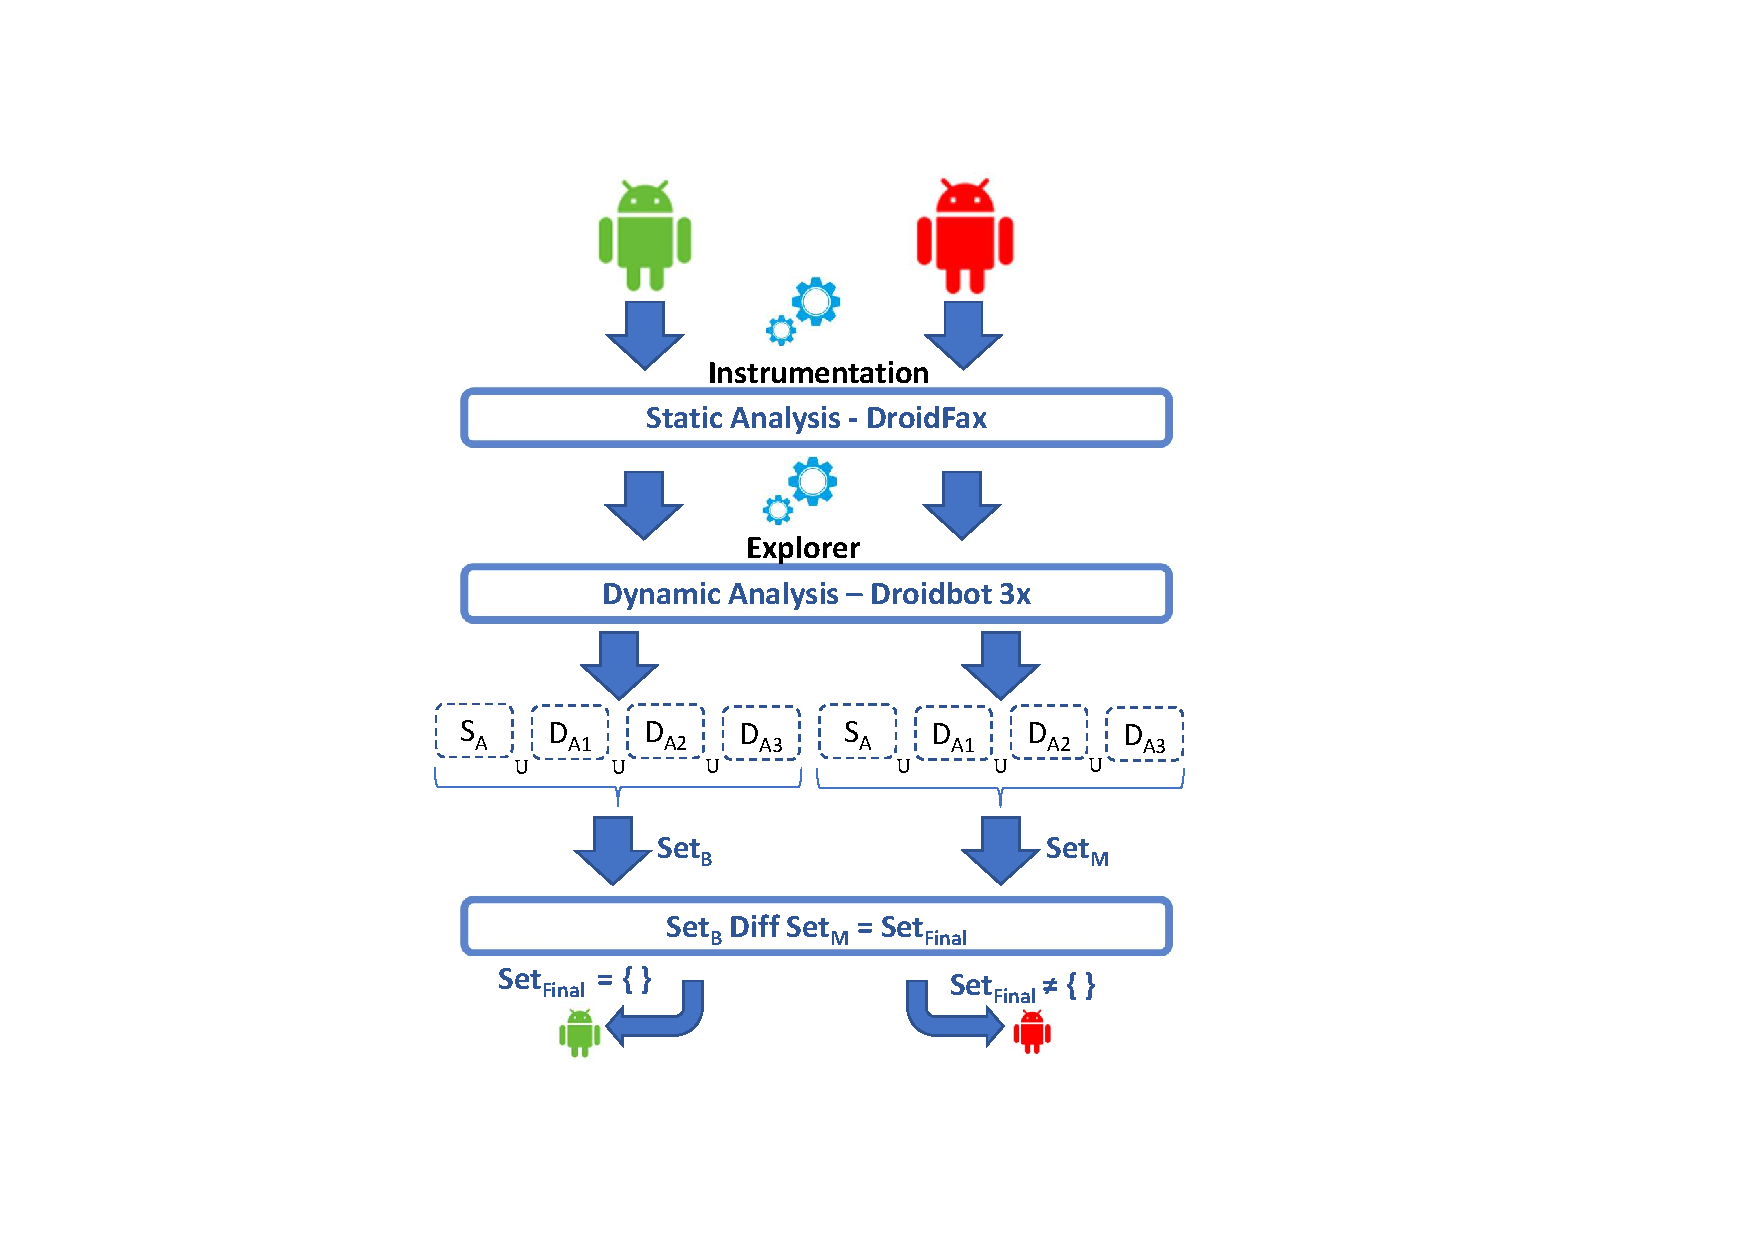
\includegraphics[width=\columnwidth]{images/mineSandbox.pdf}
  \caption{The overall architecture of the \mas}
  \label{fig:mas}
\end{figure}


\subsection{Data Analysis Procedures} \label{sec:dataAnalysisProc}



We consider that a test
generation tool, in our case, DroidBot, builds a sandbox that labels a repackaged version
of an app as a malware if there is at least one call to a sensitive APIs that (a) was observed
while executing the repackaged version of the app and that (b) was not observed while
executing the original version of the same app. If the set of sensitive methods that only the repackaged version of an app calls is empty,
we conclude that the sandbox does not label the repackaged version of an app as a malware. The set of sensitive APIs we use was defined in the AppGuard framework~\cite{DBLP:conf/esorics/BackesGHMS13}, which was based on the mapping from sensitive APIs to permissions proposed by Song et al.~\cite{DBLP:conf/ccs/FeltCHSW11}. We triangulate
the results of the \mas classification with the outputs of \vt, which might lead to one of the following
situations:

\begin{itemize}
\item {\bf True Positive (TP)}. The \mas labels a repackaged version as a malware and, according to
  \vt, at least two \ses label the asset as a malware.
  
\item {\bf True Negative (TN)}. The \mas does not label a repackaged version as a malware and,
  according to \vt, at most one \se labels the asset as a malware. 

\item {\bf False Positive (FP)}. The \mas labels a repackaged version as a malware and, according to
  \vt, at most one \se labels the asset as a malware.

\item {\bf False Negative (FN)}. The \mas does not label a repackaged version as a malware, and
  according to \vt, at least two \ses label the asset as a malware.
\end{itemize}

We compute \emph{Precision}, \emph{Recall}, and \emph{F-measure} ($F_1$) from
the number of true-positives, false-positives, and false-negatives (using standard
formulae). We use basic statistics (average, median, standard deviation) to identify the
accuracy of the \mas for malware classification, using both datasets---i.e., the \sds
with 102 pairs of apps and \cds with
\apps pairs. We use the Spearman Correlation~\cite{spearman-correlation} method and
Logistic Regression~\cite{statistical-learning} to understand the strengths of
the associations between the similarity index between the original and the repackaged versions
of a malware with the \mas accuracy---that is,
if the approach was able to correctly classify an asset as malware. We also use existing tools to reverse engineer a sample of repackaged
apps in order to better understand the (lack of) accuracy
of the \mas.


%\subsection{Environment Configuration}\label{sec:hardware}

%\todo[inline]{RB: later, if we need space, we can safely comment this section out.}

%We deployed our experiment on a 32-Core, AMD EPYC 7542 CPU, 512 GB RAM, storage Samsung SSD 970 EVO 1TB machine running a 64-bit Debian GNU/Linux 11. We also configured our emulator to run all selected apps on Google Android version 9.0, API 28, 512M SD Card, 7GB internal storage, with X86 ABI image.
%For our study, we configured DroidXP to run each of the \apps app pairs using DroidBot for 3 minutes. To mitigate noise, we repeated the full process 3 times,  which took around \review{$965$} machine hours in total. Although it was possible to run more than 10 emulators in parallel on one physical machine, to avoid any interference resulting from context switching within the operating system, we chose to run one emulator at a time. Hence, all processes took around 45 days, 40 days for experiment execution and additional 5 days for environment configuration.




\section{Results}\label{sec:results}


In this section, we detail the findings of our study.  We remind the reader that our main goal with this study is to
better understand the strengths and limitations of the \mas for malware detection using the state-of-the-art
test case generation tool (DroidBot). We explore
the results of our research using two datasets: the \sds (\appsSmall app pairs), and \cds (\apps pairs).


\subsection{Exploratory Data Analysis of Accuracy}\label{sec:accuracy}


{\bf \sds.} Considering the \sds (102 apps), the \mas for malware detection 
classifies a total of 69 repackaged versions as malware (67.64\%).
This result is close to what Bao et al. reported~\cite{DBLP:conf/wcre/BaoLL18}.
That is, in their original paper,  the \mas using DroidBot classifies 66.66\% of the
repackaged version of the apps as malware~\cite{DBLP:conf/wcre/BaoLL18}.
This result confirms that we were able to reproduce the findings of the original study using our
implementation of the \mas. 

\tb{1}{We were able to reproduce the results of
  existing research using our implementation of the \mas,
  achieving a malware classification in the
  \sds close to what has been reported in
  previous studies.}

In the previous studies~\cite{DBLP:conf/wcre/BaoLL18,DBLP:journals/jss/CostaMMSSBNR22},
the authors assume that all repackaged versions contain a
malicious behavior. For this reason, the authors do not
explore accuracy metrics (such as Precision, Recall, and
F-measure ($F_1$))---all repackaged apps labeled as
malware are considered true positives in the previous studies.
As we mentioned, in this paper we take advantage
of \vt to label our dataset and build a ground truth:
In our datasets, we classify a repackaged version of an app as malware if, according to our \vt
query results, at least two security engines identify malicious behavior in the asset.
This decision aligns with existing recommendations~\cite{vt-label,DBLP:journals/ese/KhanmohammadiEH19}).
%\kn{Now its a bit clearer, but I would expect a separate paragraph when we introduce VT explaing how VT serves as a better ground truth and also justify our choices on the numbers with VT a bit more -- why we have two as the magic number of antivirus scanners... }
The first row of Table~\ref{tab:accuracy} shows that the \mas achieves an accuracy of 0.89 when
considering the \sds. Nonetheless, the \mas fails
to correctly classify seven assets as malware on the \sds (FN column, first row of Table~\ref{tab:accuracy}),
and wrongly labeled the repackaged version of seven apps as malware (FP column).


%\kn{Please re mention in this table the total number of apps in small and complete. Maybe inside the braces as part of the second column entries. }
\begin{table*}[htb]
  \caption{Accuracy of the \mas in both datasets.}
\centering{
  \begin{tabular}{lrrrrrr} \hline
    Dataset & TP   & FP  & FN  & Precision & Recall & $F_1$ \\
    \hline
    \sds (102)    & 62   & 7   & 7   & 0.89      & 0.89   & 0.89  \\
    %\mas + Traces  & \sds (102)   & 67   & 18  & 2   & 0.78      & 0.97   & 0.87  \\
    \cds (4,076)    & 1,175  & 220 & 1,720 & 0.84       & 0.40   & 0.54  \\
    %\mas + Traces  & \cds (1203)   & 214  & 326 & 245 & 0.39      & 0.46   & 0.42  \\ 
    \hline
  \end{tabular}
  }
  \label{tab:accuracy}
\end{table*}

%We also investigate if one could improve the performance of the \mas using an enriched comparison approach. That is, instead of only comparing the sets of calls to sensitive APIs, here we also compare the traces from entry points to such a calls. If there is at least one trace that appears only during the execution of the test cases in the repackaged version of the app, we label that version as a malware.


%Introducing trace analysis reduces the number of false negatives to two, with the side effect of increasing the number of false positives from 7 to 18 (see the second row of Table~\ref{tab:accuracy}). In general, the accuracy ($F_1$) of the \mas using trace analysis drops from 0.89 to 0.87.


%\tb{2}{Although the use of Trace Analysis reduces the number of false negatives (in comparison with the vanilla \mas), it slightly decreases the overall accuracy ($F_1$) of the \mas to detect malware, from 0.89\% to 0.87\% in the \sds.} 


{\bf \cds.} Surprisingly, considering our complete dataset (\apps apps), the \mas
labels a total of \review{$1,395$} repackaged apps as malware (\review{$34.22$\%} of the total number of repackaged
apps)---for which the repackaged version calls at least one additional sensitive API.
Our analysis also reveals a {\bf negative result} related to the accuracy of the approach: here,
the accuracy is much lower in comparison to what we reported for the
\sds (see the second row of Table~\ref{tab:accuracy}): $F_1$ dropping from \fscoreSmall to \fscore.
This result indicates that, when considering a large dataset, the accuracy of the \mas using
DroidBot drops significantly.


%The use of the trace analysis reduces the number of false negatives in the \cds (from 286 to 245), though increasing the number of false positives from 173 to 326. Altogether, the $F_1$ measure does not change when comparing performance of the vanilla \mas and its trace-based variant in the \cds. 


\tb{2}{
  The \mas for malware detection
  leads to a substantially lower performance on the
  \cds (\apps pairs of apps),
  dropping the \fone from 0.89 to \fscore in comparison to
  what we observed in the \sds.}


Therefore, the resulting sandbox we generate using
DroidBot suffers from a significantly low accuracy rate when considering a large dataset.
%Besides that, enriching the \mas with trace analysis does not  improve the overall accuracy in the \cds (even though we reduce the number of false negatives with trace analysis, the increasing in the number of false positives negatively impacts the performance of the approach). 
This is shown in the second row of Table~\ref{tab:accuracy}.
The negative performance of the \mas in the \cds encouraged us to endorse efforts aimed at identifying potential reasons for
this phenomenon and motivate the research questions RQ2 and RQ3.

%\todo[inline]{The previous paragraph now seems a bit unnecessary.}

% \fh{I removed a paragraph here, since it was unncessary}

\subsection{Assessment Based on \sscore}

Figure~\ref{fig:ss} shows the \sscore distribution
over the two datasets we use in our research
(the \sds and the \cds).
Recall that the \sscore measures how similar the
original and repackaged versions of an app are.
The SmallDS exhibits an average \sscore of 0.89 (with a median of 0.99 and standard deviation of 0.25),
whereas the complete dataset averages a \sscore of 0.90 (with a median of 0.98 and standard deviation of 0.18). 

The average \sscore of the
\sds is 0.89 (median of 0.99 and sd of 0.25); while
the average \sscore of the complete dataset is
\review{0.90} (median of \review{0.98} and sd of \review{0.18}).



\begin{figure}[h]
  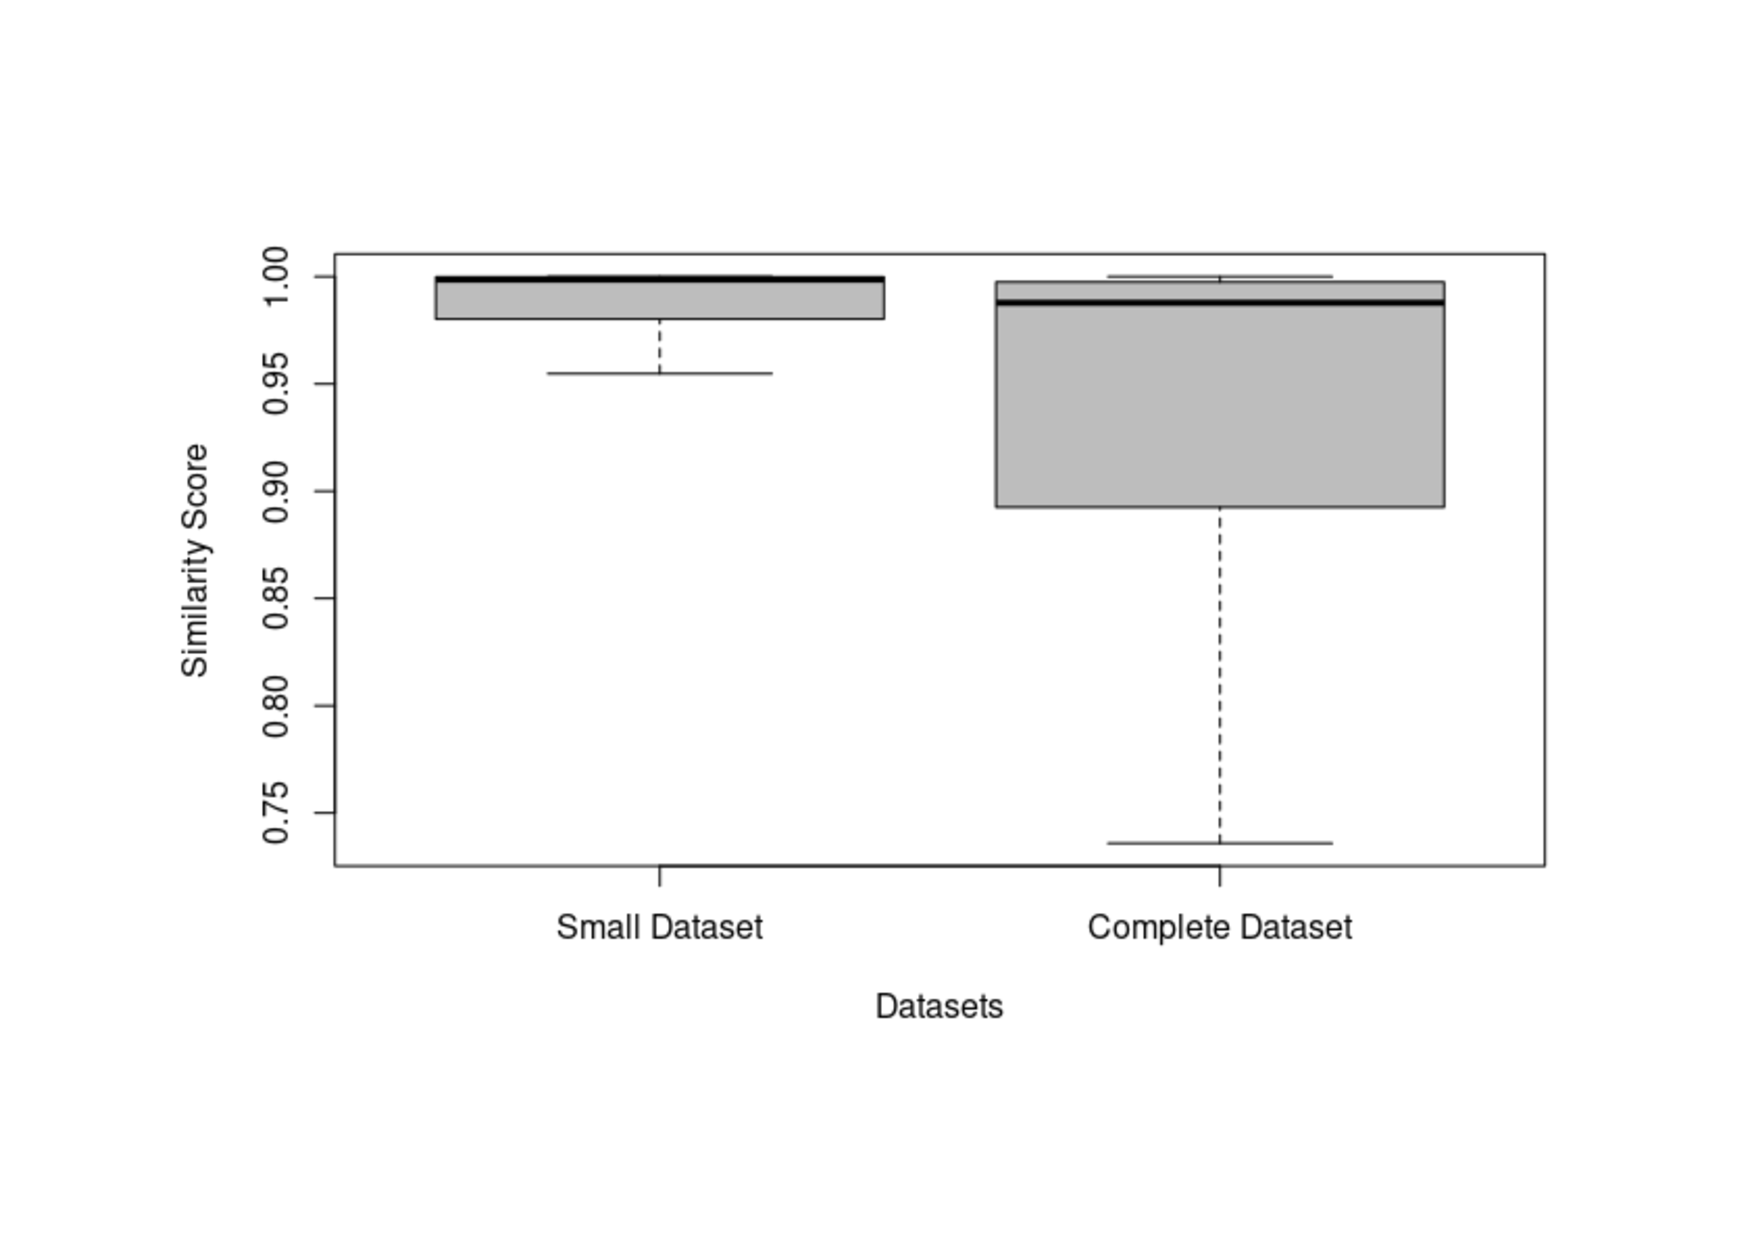
\includegraphics[width=\columnwidth]{images/boxplotSimilarity_V2.pdf}
  \caption{\sscore of the malware samples in the small and complete datasets. The boxplots in the figure do not show
  outliers.}
  \label{fig:ss}
\end{figure}



In this section we investigate how the \sscore influences the accuracy of the \mas. We employ
Logistic Regression to quantify the relationship between them. For this analysis, instances of true
negatives (i.e., cases where the repackaged version is benign according to \vt and the \mas
correctly labels it as benign) are excluded.
As such, we test the following null hypothesis:

\begin{quote}
  {\bf $H_0$} \sscore does not influence the accuracy of the
  \mas for malware detection. 
\end{quote}

The results of the logistic regression suggest that we should reject our null hypothesis ($p$-value $=$ $2.22\cdot10^{-16}$).
This finding indicates that the accuracy of the \mas is influenced by the similarity between the original and repackaged versions
of an app.


%This finding suggests that the \mas is more likely to assign a correct label to a repackaged app in the cases where its \sscore with the original app is small. %This is an expected result, since we found a higher accuracy on the \sds, even though  the \sscore of the original and repackage apps in both datasets do not differ significantly.

%\kn{I am a bit confused here. Higher similariy score implies the app pairs are close to each other, making the detection easier? Or maybe I misundertood it here.}

\tb{3}{There is an association between
  the \sscore and the \mas performance, which means that
  the similarity between the original and repackaged versions of
  an app can explain the performance
  of the \mas for malware classification.}


To clarify the lack of association between
\sscore and correctness, we use the \emph{K-Means} algorithm to split the
\cds into ten clusters---according to the \sscore. We then
estimate the percentage of correct classifications for each cluster, as
we show in Table~\ref{tab:ss-clusters}. Note that the \mas
achieves the highest percentage of correct classification (70.40\%) for the third cluster (cId = 3), which
presents an average \sscore of (0.67). Nonetheless, the
cluster cId = 10, with larger number of samples (1,248) and \sscore (0.99), presents a percentage of correct classifications of 26.68\%. We can observe that as the average similarity rate decreases, there is a tendency toward greater accuracy in the \mas. Hence, the average similarity score could explain the poor performance of the \mas on the \cds, especially considering that most samples exhibit a high average similarity of 0.99.

\begin{table}[ht]
  \caption{Characteristics of the clusters. Note there is a specific
    pattern associating the percentage of
    correct answers with the \sscore.
   For this analysis, we removed the true negatives in our dataset.}
  \centering
  \begin{small}
    \begin{tabular}{rrrrr}   \hline
 cId & \sscore & Samples & Correct Answers & \% \\ \hline

1 &  0.09 &  93 &  46 & 49.46 \\ 
  2 &  0.55 & 175 & 106 & 60.57 \\ 
  3 &  0.67 & 125 &  88 & 70.40 \\ 
  4 &  0.79 & 165 &  90 & 54.55 \\ 
  5 &  0.87 & 261 &  77 & 29.50 \\ 
  6 &  0.90 & 230 & 121 & 52.61 \\ 
  7 &  0.94 & 141 &  46 & 32.62 \\ 
  8 &  0.97 & 140 &  59 & 42.14 \\ 
  9 &  0.98 & 398 &  95 & 23.87 \\ 
  10 & 0.99 & 1248 & 333 & 26.68 \\ 
   \hline


 \end{tabular}
 \end{small}
 \label{tab:ss-clusters}
 \end{table}


\subsection{Assessment Based on Malware Family}
%\fh{inserted a little introduction about malware family}


%\kn{I feel we need some definition of what we mean by a family of malware. Words like gappusin etc donot have big meaning for people outside this domain}
As we discussed in the previous
section, the similarity assessment partially explains the low performance of the
\mas on the \cds. Since the \cds covers a wide range of malware families, we investigate the
hypothesis that the diversity of malware families in
the \cds also contributes to
the poor performance of the \mas on the \cds.
Indeed, in the \cds, we identified a total of
\review{116 malware families}, though the most frequent
ones are \gps (\appsGps samples), \fm{revmob} (207 samples), \fm{dowgin} (183 samples) and \emph{airpush} (120 samples). Together, they
account for \review{$63.79$\%} of the repackaged apps in our \cds labeled as malware according to \vt.

\review{This family distribution in the \cds is
different from the family
distribution in the \sds---where the
families \fm{kuguo} (34 samples), \fm{dowgin} (12 samples),
and \fm{youmi} (5 samples) account for
73.91\% of the families considering the 69
repackaged apps \vt labels as malware in the \sds.
Most important, in the \sds, there is just one
sample from the \gps family and no sample from \fm{revmob} family, two of the most frequent families in our \cds. This observation
leads us to the question: how does the \mas
perform when considering only samples from the \gps and \fm{revmob} families?}



The confusion matrix of Table~\ref{tab:gappusin} summarizes the accuracy assessment of the \mas considering
only the \gps and \fm{revmob} samples in the \cds. Note that \vt classifies as malware all repackaged versions in the \gps and \fm{revmob}
family. It is worth noting that the \mas failed to correctly classify
1,170 (87.5\%) samples of \gps as malware. Similarly,
92 samples (44.44\%) from \fm{revmov} were not classified as malware.
Furthermore, if we exclude the \gps and \fm{revmov} samples from the \cds,
the recall of the \mas increases to 0.72, which, although improved, remains relatively low compared to the original studies.


\begin{table}[ht]
  \caption{Confusion matrix of the \mas when considering only the
  samples from the \gps and \fm{revmob} family in the \cds.}
\centering
\begin{tabular}{r|cc} \hline
\multirow{2}{*}{Actual Condition}   & \multicolumn{2}{c}{Predicted Condition} \\ 
                                    & Benign    & Malware   \\ \hline 
  Benign   (0)                       & TN (0)    & FP (0)    \\
  Gappusin (\appsGps)                     & FN (\appsGpsFN)  & TP (167)   \\
  Revmob (207)                     & FN (92)  & TP (115)   \\
  \hline
\end{tabular}
\label{tab:gappusin}
\end{table}

\review{
  \tb{4}{The \mas fails to correctly identify 87.50\% of the samples from the \gps family and 44.44\% of
    the samples from the \fm{revmob} as malware. Just like the Similarity Score, the presence of some malware
    families with a high false negative rate also influences the low recall of the \mas in the \cds}
  }


We further analyze the samples from \gps malware family in our dataset, given its
relevance to the negative result we present in our paper, \fh{when we compare with samples from revmob family}. First, we analysed the \sscore of its samples. Figure~\ref{fig:hist-gappusin} shows a histogram of the \sscore for the samples
in the \gps family. Note that most of the repackaged versions are quite similar to the original versions (average \sscore
of 0.94, median \sscore of 0.99, and sd of 0.16). We also reengineer
a sample of 30 \gps malware, using the \texttt{SimiDroid}\footnote{https://github.com/lilicoding/SimiDroid},
\texttt{apktool}~\footnote{https://ibotpeaches.github.io/Apktool/},
and \texttt{smali2java}~\footnote{https://github.com/AlexeySoshin/smali2java} tools.
Considering this sample of 30 \gps malware, the median \sscore is 0.99. In addition,
the repackaged version of the apps changes 4.96 methods (on average). Table~\ref{tab:simidroid-outputs} summarizes
the outputs of \texttt{SimiDroid} for this sample of \gps apps.

The similarity assessment of this sample of 30 \gps malware reveals a few modification patterns when comparing the original and the
repackaged versions of the apps. First, no instance in this \gps sample dataset
modifies the Android Manifest file to require additional permissions, for instance.
In most of the cases, the repackaged version just changes the Manifest file to modify either
the package name or the main activity name. Moreover, 29 out of the 30 samples in this dataset  {\bf modifies} the 
method \texttt{void onReceive(Context,Intent)} of the class \texttt{com.games.AdReciver}. Although the results of the
decompilation process are difficult to understand in full (due to code obfuscation),
the goal of this modification is to change the behavior of the benign version, so that it can
download a different version of the \texttt{data.apk} 
asset. Figure~\ref{code:onReceive} shows
the code pattern of the \texttt{onReceive} method present in the samples. This modification
typically uses a new method (\texttt{public void a(Context)})
the repackaged versions often introduce into the same class (\texttt{AdReciver}).
Since there is no extra call to sensitive APIs, the \mas fails to label
the \gps samples correctly. 

%\begin{wrapfigure}{l}{0.4\textwidth}
\begin{figure}[h]
\centering
    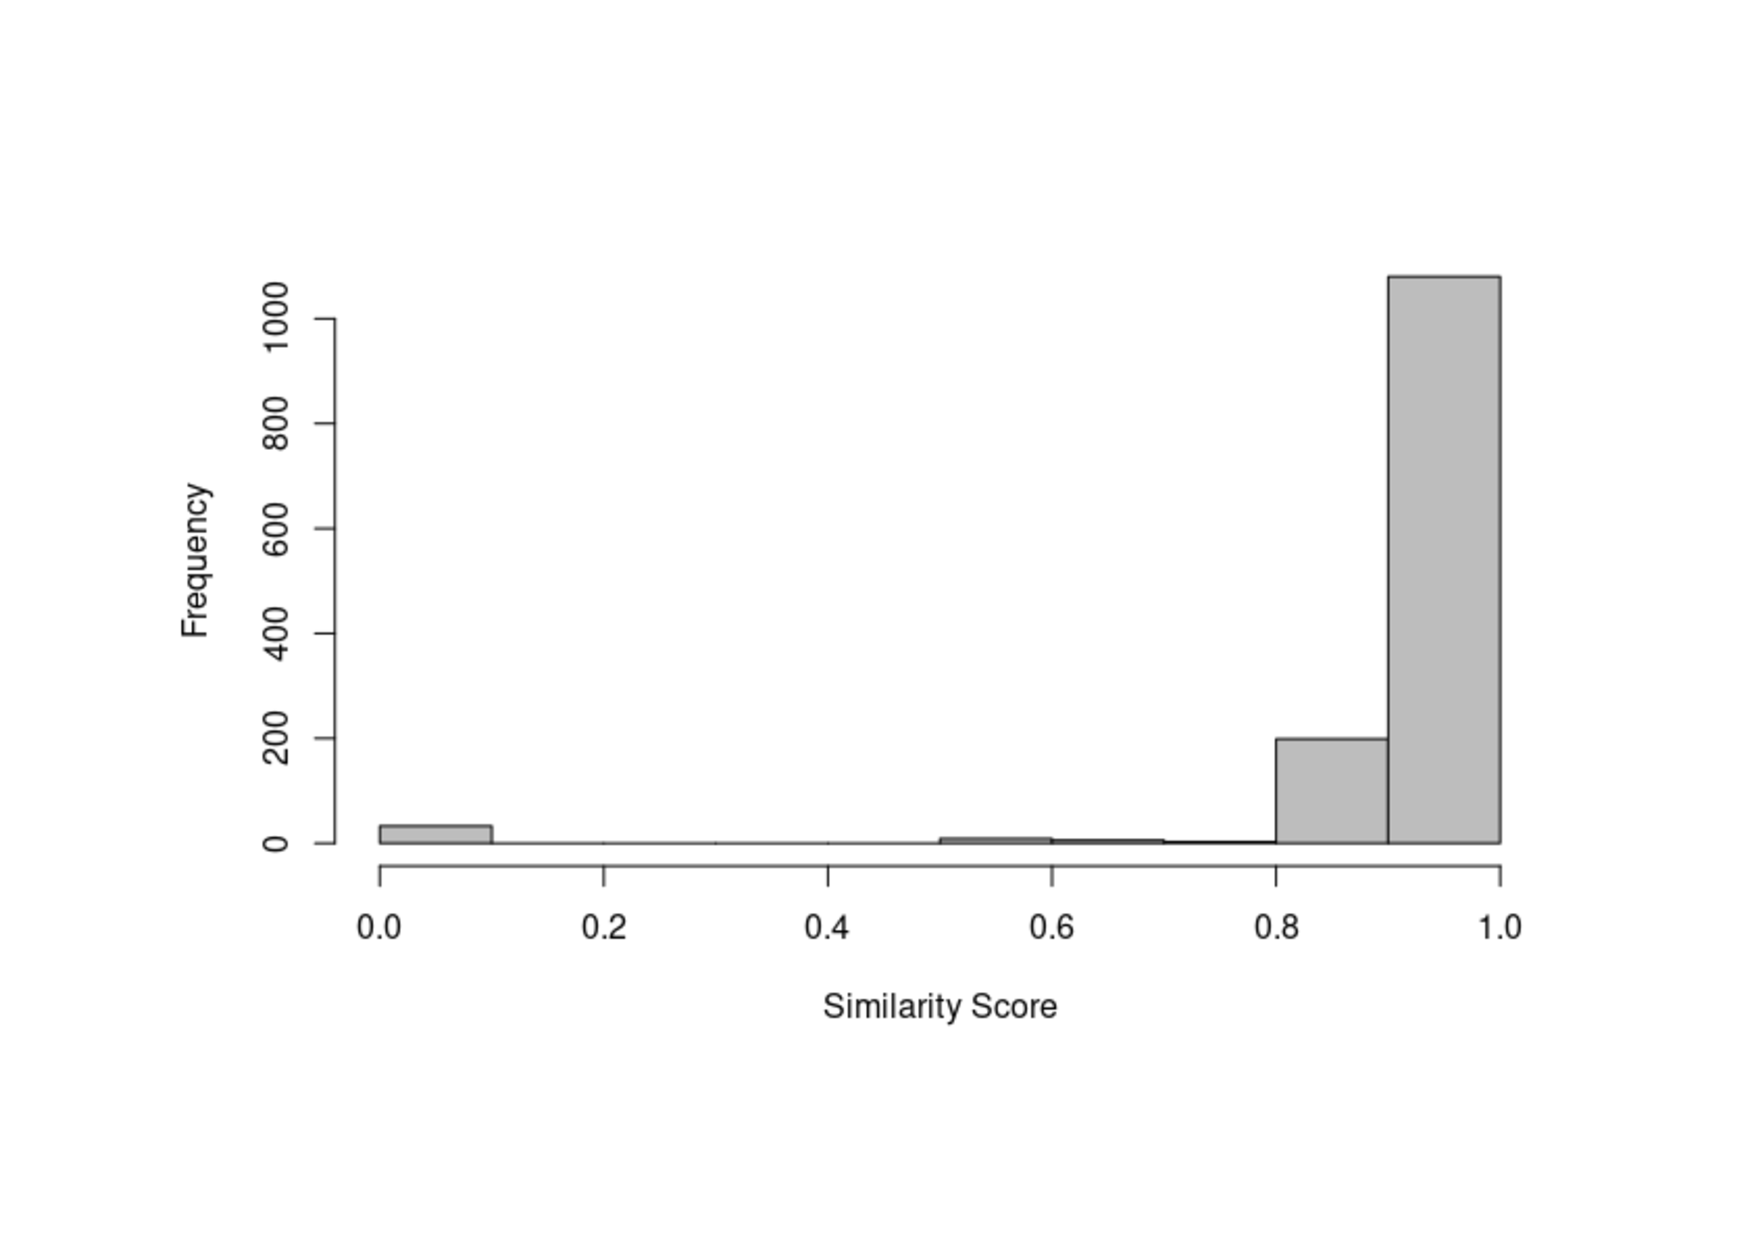
\includegraphics[width=0.7\textwidth]{images/similarityGappusin_V2.pdf}
  
  \caption{Histogram of the \sscore for the samples in the \gps family.}
  \label{fig:hist-gappusin}
\end{figure}  
%\end{wrapfigure}



\begin{figure}[h]
\centering
\lstset{texcl=true,basicstyle=\fontsize{6}{8}\selectfont\sf,commentstyle=\small\rm,mathescape=true,escapeinside={(*}{*)}}
\begin{lstlisting}[language=Java]
public void onReceive(Context context, Intent intent) {
  SharedPreferences sp = context.getSharedPreferences(String.valueOf("com.")+"game."+"param",0);
  int i = sp.getInt("sn", 0) + 1;
  System.out.println("sn: " + i);
  if (i < 2) {
    mo4a(context);
    SharedPreferences.Editor edit = sp.edit();
    edit.putInt("sn", i);
    edit.commit();
  } else if (!new C0004b(context).f7h.equals("")) {
    String str1 = context.getApplicationInfo().dataDir;
    String str2 = String.valueOf(str1) + "/fi" + "les/d" + "ata.a" + "pk";
    String str3 = String.valueOf(str1) + "/files";
    String str4 = String.valueOf("com.") + "ccx." + "xm." + "SDKS" + "tart";
    String str5 = String.valueOf("InitS") + "tart";
    String str6 = "ff048a5de4cc5eabec4a209293513b6e";    
    C0003a.m3a(context, str2, str3, str4, str5, str6);
    SharedPreferences.Editor edit2 = sp.edit();
    edit2.putInt("sn", 0);
    edit2.commit();
  }
}
\end{lstlisting}
\caption{Method introduced in 29 out of 30 \gps malware we randomly selected from the \cds.}
\label{code:onReceive}
\end{figure}

Our assessment also reveals recurrent modification patterns that {\bf delete} methods in the
repackaged version of the apps. For instance, 20 repackaged apps in our
\gps sample of 30 malware remove the method \texttt{void b(Context)} from the
class \texttt{com.game.a}. This class extensively use 
the Android reflection API. Although it is not clear the real purpose of removing these methods,
that decision simplifies the procedure of downloading a \texttt{data.apk} asset that is different
from the asset available in the original version of the apps. Removing those methods might
also be an strategy for antivirus evasion. For instance, although
some usages of the class \texttt{DexClassLoader} might be legitimate, it allows specific
types of atack based on dynamic code injection~\cite{falsina:acsac}. As such, 
antivirus might flag specific patterns using the Android reflection API suspect. 
Unfortunately, the \mas also fails to identify
a malicious behavior with this type of change (i.e., changes that remove methods).
Listing~\ref{code:deletedMethod} shows an example of code pattern frequently removed
from the repackaged versions from the \gps family. 

\begin{figure}[h]
\centering
\lstset{texcl=true,basicstyle=\fontsize{6}{8}\selectfont\sf,commentstyle=\small\rm,mathescape=true,escapeinside={(*}{*)}}
\begin{lstlisting}[language=Java]
public static void m7a(Activity activity, String str, String str2, ... , String str5) {
  try {
    Class loadClass = new DexClassLoader(..., activity.getClassLoader()).loadClass(str3);
    Object newInstance = loadClass.getConstructor(new Class[0]).newInstance(new Object[0]);
    Method method = loadClass.getMethod(str4, new Class[]{Activity.class, String.class});
    method.setAccessible(true);
    method.invoke(newInstance, new Object[]{activity, str5});
  } catch (Exception e) {
    e.printStackTrace();
  }
}  
\end{lstlisting}
\caption{Example of method that is typically removed from the repackaged apps of the \gps family.}
\label{code:deletedMethod}
\end{figure}

 
\begin{table}[ht]
  \centering
  \caption{Summary of the outputs of the \texttt{SimiDroid} tool for the sample of 30
    \gps malware. (IM) Identical Methods, (SM) Similar Methods, (NM) New Methods, and
    (DM) Deleted Methods.}
  \begin{tabular}{lrrrrr}
    \hline
 Hash  & \sscore &   IM  &   SM  &  NM   &  DM  \\ \hline
 33896E & 0.9994 &  3205 &     2 &     0 &     0 \\ 
 0C962D & 0.9994 &  3413 &     1 &     1 &    10 \\ 
 BCDF91 & 0.9992 &  2645 &     2 &     0 &     0 \\ 
 01ECE4 & 0.9991 &  5697 &     4 &     1 &    10 \\ 
 A306DA & 0.9989 &  1886 &     1 &     1 &     6 \\
 4010CA & 0.9987 &  3721 &     1 &     4 &     6 \\
 5B5F2D & 0.9983 &  1164 &     2 &     3 &     0 \\
 010C07 & 0.9982 &  2248 &     4 &     3 &     0 \\
 F9FC04 & 0.9982 &  1121 &     1 &     1 &     6 \\
 E29F53 & 0.9976 &   842 &     1 &     1 &     6 \\
 FE76EB & 0.9976 &   839 &     1 &     1 &     6 \\
 842BD5 & 0.9973 &  2249 &     3 &     3 &     3 \\
 295B66 & 0.9972 &  1081 &     2 &     1 &    10 \\
 92209D & 0.9971 &   698 &     2 &     3 &     0 \\
 0977B0 & 0.9969 &  1613 &     4 &     1 &    10 \\
 347FCF & 0.9967 &   613 &     1 &     1 &     6 \\
 00405B & 0.9965 &   864 &     2 &     1 &    10 \\
 67310E & 0.9957 &  1164 &     2 &     3 &     3 \\
 CCD29E & 0.9954 &   436 &     2 &     0 &     0 \\
 610113 & 0.9941 &   836 &     4 &     1 &    10 \\
 A871E0 & 0.9941 &   836 &     4 &     1 &    10 \\
 ECEA10 & 0.9913 &   229 &     1 &     1 &     6 \\
 E53FAA & 0.9889 &   267 &     2 &     1 &    10 \\
 723C23 & 0.9870 &   228 &     2 &     1 &    10 \\
 D95B6E & 0.9870 &   833 &    10 &     1 &    10 \\
 17722D & 0.9743 &   265 &     6 &     1 &    10 \\
 537492 & 0.9504 &   134 &     6 &     1 &    10 \\
 078E0A & 0.9504 &   134 &     6 &     1 &    10 \\
 D83F1C & 0.9494 &   150 &     2 &     6 &     6 \\
 E5D716 & 0.8840 &  2035 &    68 &   199 &   199 \\ 
   %% \texttt{0C962D289E}&0.933&99&7&0&0 \\
%% \texttt{E5D71699E7}&0.971&275&8&0&0 \\
%% \texttt{ECEA10902B}&0.897&44&5&0&0 \\
%% \texttt{5374927E98}&0.974&349&9&0&0 \\
%% \texttt{E29F53DA37}&0.986&375&5&0&0 \\
%% \texttt{BCDF919487}&0.982&334&6&0&0 \\
%% \texttt{01ECE4AE23}&0.931&108&6&2&2 \\
%% \texttt{610113BB0C}&0.964&192&7&0&0 \\
%% \texttt{295B663AD1}&0.946&196&11&0&0 \\
%% \texttt{17722D9807}&0.867&46&7&0&0 \\
%% \texttt{67310E41EC}&0.956&154&5&2&2 \\
%% \texttt{5B5F2D5DAA}&0.956&154&5&2&2 \\
%% \texttt{F9FC043249}&0.925&148&12&0&0 \\
%% \texttt{010C070CAD}&0.968&245&6&2&2 \\
%% \texttt{842BD5F8A9}&0.972&246&5&2&2 \\
%% \texttt{00405B66DD}&0.835&66&13&0&0 \\
%% \texttt{D83F1CEA61}&0.901&73&6&2&2 \\
%% \texttt{723C231BA7}&0.857&42&7&0&0 \\
%% \texttt{33896EBEC0}&0.978&229&5&0&0 \\
%% \texttt{347FCF5AC1}&0.956&110&5&0&0 \\
%% \texttt{4010CA0E70}&0.917&78&5&2&2 \\
%% \texttt{D95B6E6417}&0.981&373&7&0&0 \\
%% \texttt{A871E01516}&0.964&192&7&0&0 \\
%% \texttt{CCD29EC8ED}&0.953&102&5&0&0 \\
%% \texttt{FE76EBE7B4}&0.974&194&5&0&0 \\
%% \texttt{A306DA6482}&0.853&35&6&0&0 \\
%% \texttt{E53FAABBA0}&0.941&162&10&0&0 \\
%% \texttt{92209D0E67}&0.975&284&5&2&2 \\
%% \texttt{078E0AE6E3}&0.977&350&8&0&0 \\
%% \texttt{0977B0E411}&0.946&196&9&2&2 \\
   \hline
 \end{tabular}
 \label{tab:simidroid-outputs}
\end{table}


In summary, our reverse engineering effort brings evidence that malware samples from the \gps family neither modify the Android Manifest files nor call additional sensitive APIs. It acts as a
downloader for further malicious app~\cite{DBLP:conf/ndss/ArpSHGR14}---which reduce the ability of the \mas to correctly classify a sample as a malware. Both versions (original/repackaged) from the \gps family have the same behavior for showing advertisements to the user,
however the repackaged version have additional call sites to the advertisement API and the advertisements sources are different. This behavior is not so harmful when compared to others repackaged apps, however nothing prevents that others malware families insert malicious operations, such as theft of sensitive data.

\fh{We also analyzed three samples from the \rmb family, which were flagged by the maximum number of engines at \vt—17, 15, and 14, respectively—but were not detected by the \mas.}

%%\alert{We argue in favor of new research efforts to integrate the \mas 
%%with other techniques that could increase their performance
%%on malware identification. Since the samples from the \gps
%%family use specific patterns to introduce malicious behavior,
%%it might be promising to explore complementary techniques that
%%search for these patterns.}



 
%% \kn{I really like this part of the gps family analysis. }



%% %% \begin{figure}
%% %%   \includegraphics[scale=0.5]{images/gappusin-1.pdf}
%% %% \end{figure}

%% \todo[inline]{{\bf RB}. Removing the \gps family improves
%%   the recall, though did not improve precision. What is the reason
%%   for the low precision of \mas in the \cds? We should investigate
%% this issue.}


%% Considering
%% manifest analysis, as we explained in Section~\ref{sec:manifestAnalysis},
%% looking at the occurrence of duplicated permissions and duplicated 
%% components allows us to correctly classify \num{120} out of the \num{607} missed cases
%% from the mining sandbox approach (\num{19.76}\%).                                   
%% Table~\ref{tab:mfa-complete} summarizes the results of this investigation. When considering the 
%% complete dataset (\num{800} apps), combining the vanilla
%% mining sandbox approach (VMS) with trace analysis (TA) and
%% manifest analysis (MA) leads to the correct classification
%% of \num{446} malware (\num{55.75}\%), which suggests that
%% the mining sandbox approach requires further improvements when
%% we take into account a more representative dataset
%% of malware. 


%% \begin{table}[ht]
%%   \centering
%%   \begin{small}
%%   \begin{tabular}{lcc}\toprule
%%   Technique      & Hits & Recall \\ \midrule 
%%   VMS            & 193  & \num{24.12}\% \\ 
%%   VMS + TA       & 369  & \num{46.12}\%  \\
%%   VMS + MA       & 313  & \num{39.12}\% \\
%%   VMS + TA + MA  & 446  & \num{55.75}\% \\  \bottomrule
%%   \end{tabular}
%%   \end{small}
%%     \caption{Summary of the results in the Complete Dataset.}

%%  \label{tab:mfa-complete}
%% \end{table}

%% \begin{obs}{5}{}
%%   The results so far bring evidence that
%%   further research is necessary to understand
%%   the limitations of the mining sandbox approach
%%   targeting more comprehensive datasets.
%% \end{obs}

%% Our exploration of all sensitive APIs called by all app pairs brought to the light the most frequently abused sensitive APIs that
%% appear in the repackaged, malicious version of the apps. We observed that when executed all 800 app pairs, DroidBot called $75$ sensitive APIs at least one time (from our list of 162 sensitive APIs). Among them, $16$ APIs account for more than half of all calls ($51.06$\%).
%% %\rb{I could not understand the previous sentence}.
%% The sensitive API that is abused the most by repackaged apps is \textbf{android.telephony.TelephonyManager: java.lang.String getDeviceId()}, which gets the device
%% IMEI\footnote{From Wikipedia: International Mobile Equipment Identity (IMEI) is a number, usually unique, to identify 3GPP and iDEN mobile phones.}.
%% Table~\ref{tab:APIused} presents the list of the most frequent sensitive APIs that only the malicious
%% version of the apps in our dataset call.

%% \begin{obs}{6}{}
%%   The results so far bring evidence that only a handful of resources accesses like the \textbf{device id} are most attractive to malware designers, providing a potentially high-impact point of focus for future researchers and practitioners.
%% \end{obs}

%% %\begin{landscape}
%% \begin{table*}[t]
%%  \scriptsize
%%   \caption{Sensitive APIs more used by repackage apps}
%%   \centering
%%   %\begin{small}
%%  \begin{tabular}{lc}

%%    \toprule
%%    Sensitive API & Occurrences \\
%%    \midrule
%%    01 android.telephony.TelephonyManager: java.lang.String getDeviceId() &  78 \\
%%    02 android.net.wifi.WifiManager: android.net.wifi.WifiInfo getConnectionInfo() &  64\\
%%    03 android.net.wifi.WifiInfo: java.lang.String getMacAddress() &  63 \\
%%    04 android.net.NetworkInfo: java.lang.String getTypeName() &  58 \\
%%    05 android.net.NetworkInfo: java.lang.String getExtraInfo() &  56 \\
%%    06 android.telephony.TelephonyManager: java.lang.String getSubscriberId() &  54 \\
%%    07 android.net.NetworkInfo: android.net.NetworkInfo State getState() &  52 \\
%%    08 android.database.sqlite.SQLiteOpenHelper: android.database.sqlite.SQLiteDatabase getWritableDatabase() &  49 \\
%%    09 android.database.sqlite.SQLiteDatabase: android.database.Cursor query(java.lang.String, ...,java.lang.String) &  47 \\
%%    10 android.telephony.TelephonyManager: java.lang.String getNetworkOperator() &  45\\
%%    11 android.telephony.TelephonyManager: android.telephony.CellLocation getCellLocation() &  44\\
%%    12 android.database.sqlite.SQLiteOpenHelper: android.database.sqlite.SQLiteDatabase getReadableDatabase() &  44\\
%%    13 android.telephony.gsm.GsmCellLocation: int getLac() &  42 \\
%%    14 android.telephony.gsm.GsmCellLocation: int getCid() &  42 \\
   
%%    15 android.net.ConnectivityManager: android.net.NetworkInfo getNetworkInfo(int) &  39 \\
%%    16 android.telephony.TelephonyManager: java.lang.String getNetworkOperatorName() &  36 \\
%%    .&  .\\
%%    .&  .\\
%%    .&  .\\
%%    74 android.app.ActivityManager: java.util.List getRecentTasks(int,int) & 1 \\
%%    75 android.net.NetworkInfo: java.lang.String toString() & 1 \\

%%  \bottomrule
%%                             Total & 1592 \\

%%  \end{tabular}
%%  %\end{small}
%%  \label{tab:APIused}
%% \end{table*}
%\end{landscape}

%% \begin{obs}{1}{}
%%    %\kn{Here we need to add some final take aways of the reproduction study}
%%    Our results indicate that in the presence of a representative dataset ($800$ app pairs as opposed to $102$ and a diverse similarity index), the accuracy of state of the art in mining sandbox approaches, using DroidBot drops significantly (from $63.36\%$ to $24.12\%$). Our results also indicate that only few sensitive APIs are responsible for majority of injected malware in repackaged apps. This encourages the emergence of new proposals that can support mine sandbox mitigating \textit{blindspot}s that lead to low accuracy.
%%  \end{obs}


%\kn{In this subsection, are we simply reproducing the results of existing papers. Because as far as I understand, tools like DroidBOT etc. were evaluated by simply comparing the sensitive APIs call. I am guessing here our contribution is to evaluate it on the larger dataset. I have given it a shot, please keep me posted if this is correct.}

%% \subsection{Trace Analysis Results}\label{sec:traceResults}

%% In this section, we describe the results of our investigation on how the trace from the entry point to sensitive API could impact the accuracy of sandbox approaches. Initially, we collect the call graphs of DroidBot execution using \emph{Logcat} and filter in the traces between the app's entry point and calls to any sensitive methods.

%% Then, using the callgraph from executions of both app versions (benign/malicious), we track the differences between their traces. We choose to investigate only app pairs that covered the same set of sensitive APIs detected in both versions during our first experiment (Section~\ref{sec:Sensitive APIs}). 


%% \begin{obs}{2}{}
%%  The state of the art in mining sandbox approaches using DroidBot have a blind-spot when it comes to being aware of the trace taken from the entry point to a sensitive API call. The approaches could have a improvement of $22\%$ if it considered trace as a factor. Similar  improvements are also seen with the original dataset of $101$ app pairs (improvement of $18.81\%$).
%%  \end{obs}

%% \subsection{Manifest File Analysis}\label{sec:manifestResults}

%% In this section, we describe the results of our investigation on the impact of modified manifest files on the accuracy of sandbox approaches. 
%% To this end, we check some particulars from manifest file, that point to a likely suspicious behavior. In section \ref{sec:manifestAnalysis}, we illustrated that an automatic hacking script could inject permission requests at manifest file regardless of whether this request is already present on it, which can result in duplicated permission and actions in the Manifest file. We looked out for such modifications in the malware that went undetected by the test generation tools. Table~\ref{tab:mfa} summarizes our results.


%% The column (SAPI) indicates the number of malware that went undetected during our first study (same as Table~\ref{tab:pa}'s Same API set (SAPI)). The second column (DP) indicates how many Manifest files from malicious app undetected at first study, had duplicated permission. Same way, column (DA) denotes the number of Manifest files with the duplicated actions in their manifest file.

%% A duplicate request for permission or action in a malicious version's manifest file should have been performed by a script. A simple analysis of manifest file could detect $120$ of undetectable malware from the first experiment ($607$), if it considers explorer duplicate permissions or actions at manifest file code as a detection strategy. If we combine the previous trace analysis with manifest file analysis, we improve the accuracy rate to $55.75\%$.

%% It is to be noted that in the presence of the original dataset of $101$ app pairs, the manifest file analysis combined with the trace analysis earlier discussed improves the accuracy rate to $90.09\%$ confirming that such an analysis, even though naive and simple does have an impact on the accuracy rate of mining sandbox approaches.  %\kn{Handrick as before please put the full numbers in the table}


%% \begin{obs}{3}{}
%%  We can conclude that sandbox approach also could have better accuracy if they considered the suspicious modifications in manifest file in their analysis. Although the analysis required of the manifest file is quite naive, we believe the results present an interesting and relevant insight for developers of malware detection tools to improve accuracy.
%% \end{obs}

%% \todo[inline]{rb: I reviewed the paper until this point. I think that next we should
%% provide more explicit answers to the research questions. kn: Given this a shot}

%% \todo[inline]{mm: any finding we want to formulate related to the discussion in the last paragraph? kn: Given it a shot}


\section{Discussion}\label{sec:discussion}

In this section, we answer our research questions,
summarize the implications of our results, and discuss possible
limitations of our study that might threaten the
validity of the results presented so far.

\subsection{Answers to the Research Questions}

The results we presented in the previous sections
allow us to answer our three research questions, as
we summarize in the following.

\begin{itemize}
\item \textbf{Performance of the \mas on the \cds (RQ1).} 
  Our study indicates that the accuracy of the \mas reported in
  previous studies~\cite{DBLP:conf/wcre/BaoLL18,DBLP:journals/jss/CostaMMSSBNR22} does not
  generalize to a larger dataset. That is, while in our
  reproduction study (using the \sds of previous research) the \mas
  leads to an accuracy of \fscoreSmall, we observed a drop of precision and recall
  that leads to an accuracy of \fscore in the presence of our \cds (\apps pairs of
  original and repackaged versions of Android apps). 

%\item \textbf{Effect of trace analysis (RQ2).} We do not find any gain of enriching the vanilla \mas with trace analysis in terms of accuracy ($F_1$ score). Although the use of traces reduces the number of false negatives (improving recall), it also increases the number of false positives with a similar proportion---which does not change the $F_1$ score significantly. Nonetheless, for the context of malware identification, we believe that the gain in terms of recall might justify the use of trace analysis.

\item \textbf{Similarity Analysis (RQ2).} Our results bring evidence about the existence of an association between the similarity of the original and repackaged versions of an app and the ability of the \mas to correctly classify a repackaged version of an app as a malware. Therefore, the similarity assessment can explain the low performance of the \mas to identify malware in the \cds.
\review{
\item \textbf{Malware Family Analysis (RQ3).} The results indicate that some families are responsible for the largest number of false negatives in the complete dataset. We specifically further investigate the \gps family, which corresponds to a particular type of
Adware, designed to automatically display advertisements while an app is running. After reverse engineering a sample of 30 \gps malware, we confirmed that the \mas cannot identify the patterns of changes introduced in the repackaged versions of the apps. The prevalence of the \gps family in the \cds also contributed to explaining the poor performance of the \mas for malware classification in the large dataset.}



\end{itemize}



Although some families explains the drop in the recall of the \mas, other reasons might explain the reduced precision of the \mas in the \cds. First, the distribution of samples equally between families in the datasets might partially explain the low precision of the \mas in the \cds. Second, we only label a repackaged version of an app as malware if \vt reports that at least two engines find suspicious behavior in that asset. This decision might be considered an over-constraint. \fh{However, when we relax this constraint and label an asset as malware whenever at least one engine detects suspicious behavior, despite improving precision to 0.85, we decrease recall to 0.39. In general, the accuracy of the \mas remain the same 0.53---still significantly smaller than the \mas precision for the \sds. Although previous research suggests that two engines is a reasonable threshold for labeling an app as malicious, we also checked the accuracy when considering five and ten engines. We obtained similar results, with accuracy no higher than 0.55. The accuracy for each engines is show in Table~\ref{tab:engines}.}

\begin{table*}[htb]
  \caption{Accuracy of the \mas at \cds (4,076 pairs) based on engines.}
\centering{
  \begin{tabular}{lrrrrrr} \hline
    Engine(s) & TP   & FP  & FN  & Precision & Recall & $F_1$ \\
    \hline
    At least 01    & 1,222  & 220 & 1,900 & 0.85       & 0.39   & 0.53  \\
   
    At least 02    & 1,175  & 220 & 1,720 & 0.84       & 0.40   & 0.54  \\
   
    At least 05    & 1,087  & 220 & 1,578 & 0.83       & 0.40   & 0.54  \\
   
    At least 10    & 1,002  & 220 & 1,469 & 0.81       & 0.40   & 0.54  \\
    \hline
    
  \end{tabular}
  }
  \label{tab:engines}
\end{table*}




\begin{comment} First, the proportion of malware samples in the
datasets differs. That is, \vt labels \review{$66.95$\%} of the repackaged version of the apps in the \cds as malware---contrasting with 67.64\% of the samples that \vt labels as malware in the \sds.
\end{comment}

\subsection{Implications}\label{sec:implications} 

Contrasting to previous research works~\cite{DBLP:conf/wcre/BaoLL18,DBLP:conf/iceccs/LeB0GL18,DBLP:journals/jss/CostaMMSSBNR22},
our results 
%discussed in the previous sections 
lead to a more systematic understanding
of the strengths and limitations of using the \mas
for malware classification. In particular, this is the
first study that empirically evaluates the \mas
considering as ground truth the outcomes
of \vt. This decision allowed us to explore the
\mas performance using well-known accuracy metrics (i.e., precision, recall, and
$F_1$ score). Previous studies assume that all repackaged versions of the
apps were malware. Our triangulation with \vt reveals this is not true. Although
the \mas presents a good accuracy for the \sds ($F_1$ = \fscoreSmall), 
in the presence of a large dataset the \mas accuracy drops significantly ($F_1$ = \fscore). 

\review{We also reveal that some families in the \cds are responsible for a large number of false negatives,
compromising the accuracy of the \mas.
Altogether, the takeaways of this research are twofold:}

\begin{itemize}
  \item Negative result: the \mas for malware detection exhibits a much higher false negative rate than previous research reported. 

  \item Future directions: Researchers should advance the \mas for malware detection by exploring more advanced techniques for differentiating between benign and malicious versions of the apps. In particular, new approaches should benefit from techniques that can identify specific patterns of changes in the repackaged versions and mine sensitive calls to native APIs. The state-of-the-art on mining sandbox ignore native calls.
    
\end{itemize}  


\subsection{Threats to Validity}\label{sec:threats}

% \todo[inline]{MM: Needs major revision.}

There are some threats to the validity of our results.
Regarding {\bf external validity}, one concern relates to the 
representativeness of our malware datasets and how generic our findings are.
Indeed, mitigating this threat was one of the motivations for our research,
since, in the existing literature, researchers had explored just
one dataset of 102 pairs of original/repackaged apps. Curiously,
for this small dataset, the performance of the
\mas is substantially superior
than its performance on our \cds (\apps pairs of
apps).

We contacted the authors of the Bao et al. research paper~\cite{DBLP:conf/wcre/BaoLL18}, asking them
if they had used any additional criteria for selecting the pairs of apps in their
dataset. Their answers suggest the contrary: they have not used
any particular app selection process that
could explain the superior performance of the \mas for the \sds. We believe that
our results in the \cds generalize better than previous research work,
since we have a more comprehensive collection of malware with different
families and degrees of similarity. Nonetheless, our
research focus only on Android repackaged malware and thus we cannot generalize
our findings to malware that targets other platforms or that use different approaches
to instantiate a malicious asset. Besides that, repackaging is a recurrent approach
for implementing Android malware.

Regarding {\bf conclusion validity}, during the exploratory phase of the \mas, we collected the set of calls to sensitive APIs the original version of
an app executes, while running a test case generation tool (DroidBot).
That is, the \mas assumes the existence of a benign original
version of a given app in the exploratory phase. \highlight{We also query \vt to confirm this
assumption, and found that the original version of seven (out 102) apps in the
\sds contains malicious code. We believe the authors of previous studies carefully check that assumption,
and this difference had occurred because the outputs of \vt change over time~\cite{vt-label}}, and a dataset that is consistent at a date will
not so in the future.
Therefore, while reproducing this research, it is necessary to query \vt to get the most up-to-date classification of the assets, which might lead to results that might slightly
diverge from what we have reported here. Besides that, in the \cds we only consider
pairs of original/repackaged apps for which \vt classifies the original version as benign. 

\begin{comment}    
Regarding the \textbf{correlation between dataset properties and accuracy drop}, after running statistical tests (logistic regression),
we could not find evidence that the \emph{diversity} of the
complete dataset---in terms of similarity score and types of malware-
is responsible for the higher number of false negatives of the mining
sandbox approach. This implies that there was no 1-1 correlation between the brackets of similarity index, malware types to the drops in accuracy. Therefore, further research is necessary to investigate
other possible reasons for that. Perhaps, the complete dataset
contains a large percentage of malware that use more
advanced techniques to evade from both static and dynamic analysis---
both methods are used in the mining sandbox approach
we discussed in this paper.
\end{comment}


Regarding {\bf construct validity}, we address the main threats to our study by using simple and
well-defined metrics that are in use for this type of research: number of malware samples the
\mas correctly/wrongly classify in a dataset (true positives/false negatives).
Based on these metrics, we computed the accuracy results using precision and recall. In a preliminary study, we
investigated whether or not the \mas would classify an original version of an app as a malware,
computing the results of the test case generation tools in multiple runs. After combining three executions
in an original version to build a sandbox, we did not find any other execution that could wrongly
label an original app as a malware. 

%\section{Conclusions and Future Work}\label{sec:conclusions}
\section{Conclusions}\label{sec:conclusions}


To better understand the strengths and limitations of the \mas for repackaged malware detection, this paper reported the results of an empirical study that reproduces previous research works~\cite{DBLP:conf/wcre/BaoLL18,DBLP:journals/jss/CostaMMSSBNR22} using a more diverse dataset---in comparison to the datasets used in previous research. To our surprise, compared to published results, the performance of the \mas drops significantly for our comprehensive dataset ($F_1$ score reduces from 0.89 in previous papers to 0.54 here). This result is partially explained by the high prevalence of a specific malware families (named \gps and \rmb), whose samples are incorrectly classified by the \mas. We also report the results of a reverse engineering effort, whose goal was to understand the features from the \gps and \rmb family that reduce the performance of the \mas for malware classification. Our reverse engineering effort revealed common changing patterns in the \gps repackaged versions of original apps, which mostly use reflection to download an external apk asset for handling advertisements without introducing additional calls to sensitive APIs. \fh{Similarly, the \rmb family does not include any additional calls to sensitive resources, however it often uses JNI to interact with native code, which can be used to perform malicious operations at a low level, compromising the effectiveness of the \mas for malware identification. These negative results highlight the current limitations of the MAS approach for malware classification and suggest the need for further research to integrate the MAS approach with other techniques for more effective malware identification.}






%Additionally, the low $F_1$ score is also driven by the reduced precision rate of the \mas in the \cds. The high number of false positives explains this low rate, and has a possible explanations, our imbalance dataset, since \vt labels few samples in the \cds as malware. We open discuss about the number of engines we must consider for \vt report a repackage as malware, since the stricter we were in this criterion, the precision of the \mas down.


\balance 


\bibliography{ref}



\end{document}

